\chapter[Dynamic Programming]
{Dynamic Programming (DP)
  \label{chDynmcPrgrmmng}}
\chaptermark{Dynamic Programming}

When doing ``5. Longest Palindromic Substring'', I still have a bit of
problem with dynamic programming. So here are my own notes.


\section{Dynamic Programming---From Novice to Advanced
  \label{secDynmicPrgrmmngFrmNvcToAdvncd}}

\url{https://www.topcoder.com/community/data-science/data-science-tutorials/dynamic-programming-from-novice-to-advanced/}

By Dumitru---topcoder member

An important part of given problems can be solved with the help of dynamic
programming (\textbf{DP} for short). Being able to tackle problems of this
type would greatly increase your skill. I will try to help you in
understanding how to solve problems using DP. The article is based on
examples, because a raw theory is very hard to understand.

Note: If you're bored reading one section and you already know what's being
discussed in it---skip it and go to the next one.

\subsection{Introduction (Beginner)
  \label{subsecDPIntro}}

\rrheader{What is a dynamic programming, how can it be described?}

A \textbf{DP} is an algorithmic technique which is usually based on a
recurrent formula and one (or some) starting states. A sub-solution of the
problem is constructed from previously found ones \rrblue{(I think CLRS
  refers to states as structures. So we have to identity the optimal
  substructure which gives raise to the optimal solution. Thus, DP relies on
  the fact that an optimal solution can be constructed from optimal
  sub-solutions.)}. DP solutions have a polynomial complexity which assures
a much faster running time than other techniques like backtracking,
brute-force etc.

Now let's see the base of DP with the help of an example:

Given a list of $N$ coin \rrblue{(types)}, their values ($v_1$, $v_2$,
$\ldots$ , $v_N$), and the total sum $S$.  Find the minimum number of coins
the sum of which is $S$ (we can use as many coins of one type as we want),
or report that it's not possible to select coins in such a way that they sum
up to $S$.

Now let's start constructing a DP solution:

First of all we need to find a state for which an optimal solution is found
\rrblue{(i.e. the optimal sub-structure)} and with the help of which we can
find the optimal solution for the next state \rrblue{(so the optimal
  solution is created using the optimal sub-solution)}.

\rrheader{What does a ``state'' stand for?}

It's a way to describe a situation, a sub-solution for the problem. For
example a state would be the solution for sum $i$, where $i\leq S$
\rrblue{(i.e. a sub-structure which provides the optimal sub-solution for
  $i$, where $i\leq S$)}. A smaller state than state $i$ would be the
solution for any sum $j$, where $j<i$. For finding a state $i$, we need to
first \textbf{find all smaller states $\bm{j}$} ($j<i$) . Having found the
minimum number of coins which sum up to $i$, we can easily find the next
state---the solution for $i+1$.

\rrheader{How can we find it?}

It is simple---\rrhl{for each} coin $j$, with value $v_j\leq i$
\rrblue{(note that the value has to be less than $i$, since, e.g. we cannot
  create a sum $5p$ with a $10p$ coin)}, look at the minimum number of coins
found for the $i-v_j$ sum (we have already found it previously). Let this
number be $m$. If $m+1$ is less than the minimum number of coins already
found for current sum $i$, then we store this new result for it.
\rrblue{(This makes sense. See below.)}

\RayNotesBegin

Okay, this makes sense now (after I've seen the code). Now I will describe a
problem and how to solve it. The next section does more or less the same
thing but I think I can explain it better.

Say we have three coin types with values: $v = \brce*{v_1 = 1, v_2 = 3, v_3
  = 5}$, we want to minimize the number of coins required to make $S=11$.

First we have to think can we construct an optimal solution from an optimal
sub-solution? Say we have to solve for sum $i<S$, and we already obtained
the optimal sub-solutions for sums less than $i$. Then we simply work
through the coin types $\brce*{v_1..v_3}$ and say, if the solution to sum
$i$ contains coin $v_1$, what other coins should it contain? Well, $i - v_1
= k$ is the left over sum. So we look at the optimal value we've calculated
for $k$. Since we know we have used one coin already (in this case, $v_1$),
the solution would be the solution for $k$ plus $1$. And we keep doing this
with the rest of the coin types for this sum $i$, and update the most
optimal solution we've found so far.

Key take aways:
\begin{itemize}%[noitemsep,topsep=0pt]
\item Identified that we can create the solution to sum $i$ by using coin
  type $v_j$ (which gives us one coin) plus the solution obtained for sum
  $i-v_j$.
\item We work this out for all coin types $v_j$, and store/update the
  solution for $i$.
\item That's basically it. We're working from left to right of the sums:
  $0\leq i\leq S$, and at each step $i$, we know we've already calculated
  the optimal solution for $k<i$.
\end{itemize}

\RayNotesEnd

For a better understanding let's take this example \rrred{(yes, please do)}:
\begin{quotation}
Given coins with values $1$, $3$, and $5$.\\
And the sum $S$ is set to be $11$.
\end{quotation}

\begin{itemize}%[noitemsep,topsep=0pt]
\item First of all we note that for state 0 (sum $i=0$) we have found a
  solution with a minimum number of 0 coins.
\item \textbf{We then go to sum $\bm{i=1}$:}. First, we note that we haven't
  yet found a solution for this one (a value of $\infty$ would be a good
  sentinel, since we are trying to find the min. number of coins). 

  Now we work through the coins $j$. Then we see that only coin 1 is less
  than or equal to the current sum $i=1$.

  \begin{itemize}%[noitemsep,topsep=0pt]
  \item \textbf{Coin $j=1$, $v_1=1$:} Now we we see that for sum
    $i-v_1=1-1=0$, we have a solution with $0$ coins. Because we add one
    coin to this solution \rrblue{(since we used one coin of value $v_1 =
      1$)}, we'll have a solution with $1$ coin for sum $1$. It's the only
    solution yet found for this sum.  We write (save) it \rrblue{(in a table
      or something, so we can easily look up how many coins are needed to
      make value $i$)}.
  \end{itemize}
\item \textbf{Then we proceed to the next state---sum $\bm{i=2}$:}. We 
  again see that the only
  coin which is less or equal to this sum $i=2$ is the first coin, having a 
  value of $v_1 = 1$. So for each coin $j$:
  \begin{itemize}%[noitemsep,topsep=0pt]
  \item \textbf{Coin $j=1$, $v_1=1$:} The optimal solution found for sum
    $i-v_1=2-1=1$ is $1$ coin. This coin plus the first coin \rrblue{(the
      $v_1$ we just took off)} will sum up to $2$, and thus make a sum of
    $2$ with the help of only $2$ coins. This is the best and only solution
    for sum $i=2$.
  \end{itemize}
\item Now we proceed to sum $i=3$. We now have 2 coins which are to be
  analyzed---first $j=1$ \rrblue{(with value $v_1=1$)} and second one
  \rrblue{(with value $v_2=3$)}. Let's see the first one.
  \begin{itemize}%[noitemsep,topsep=0pt]
  \item \textbf{Coin $j=1$, $v_1=1$:} There exists a solution for sum
    $2=i-v_1=(3-1)$ and therefore we can construct from it a solution for
    sum $i=3$ by adding the first coin \rrblue{($j=1$ with $v_1=1$)} to it
    \rrblue{(``\emph{it}'' being the solution, so now the solution consists
      of one coin)}.  Because the best solution for sum $i=2$ that we found
    has $2$ coins, the new solution for sum $i=3$ will have $3$ coins
    \rrblue{(since the solution already has one coin)}.
  \item \textbf{Coin $j=2$, $v_1=3$:} Now let's take the second coin with
    value equal to $3$. The sum for which this coin needs to be added to
    make $i=3$ , is $i-v_2=3-3=0$. We know that sum $i=0$ is made up of $0$
    coins. Thus we can make a sum of $3$ with only one coin---$3$. We see
    that it's better than the previous found solution for sum $3$, which was
    composed of $3$ coins. We update it and mark it as having only $1$ coin.
  \end{itemize}
\item The same we do for sum $i=4$, and get a solution of $2$ coins ---
  $1+3$ \rrblue{(or $2+2$)}. And so on.
\end{itemize}

Pseudocode:
\begin{lstlisting}[style=pseudostyle]
Set Min[i] equal to Infinity for all of i
Min[0]=0

For i = 1 to S
  For j = 0 to N - 1
    If (Vj<=i AND Min[i-Vj]+1<Min[i])
      Then Min[i]=Min[i-Vj]+1

Output Min[S]
\end{lstlisting}

Here are the solutions found for all sums:

\begingroup
\renewcommand*{\arraystretch}{\arraystretchsize}
\begin{footnotesize}
\begin{longtable}{|l|p{2.5cm}|p{9cm}|}
% header and footer information
\hline
\endfirsthead
\hline
\endlastfoot
% body of table
Sum &Min. nr. of coins&Coin value added to a smaller sum to obtain his sum
(it is displayed in brackets)\\\hline
0&0&-\\\hline
1&1&1 (0)\\\hline
2&2&1 (1)\\\hline
3&1&3 (0)\\\hline
4&2&1 (3)\\\hline
5&1&5 (0)\\\hline
6&2&3 (3)\\\hline
7&3&1 (6)\\\hline
8&2&3 (5)\\\hline
9&3&1 (8)\\\hline
10&2&5 (5)\\\hline
11&3&1 (10)\\
\end{longtable}
\end{footnotesize}
\endgroup

Code for this is in:\\
\path{src/DynamicProgramming/rrrMinCoinSum.cpp}

As a result we have found a solution of 3 coins which sum up to 11.

Additionally, by tracking data about how we got to a certain sum from a
previous one, we can find what coins were used in building it. For example:
to sum $i=11$, we got by adding the coin with value 1 to a sum of $i=10$. To
sum $i=10$ we got from $5$. To $i=5$---from $0$. This way we find the coins
used: $1$, $5$ and $5$.

Having understood the basic way a DP is used, we may now see a slightly
different approach to it. It involves the change (update) of best solution
yet found for a sum $i$, whenever a better solution for this sum was found.
In this case the states aren't calculated consecutively. Let's consider the
problem above. Start with having a solution of $0$ coins for sum $0$. Now
let's try to add first coin (with value $1$) to all sums already found. If
the resulting sum $t$ will be composed of fewer coins than the one
previously found---we'll update the solution for it. Then we do the same
thing for the second coin, third coin, and so on for the rest of them. For
example, we first add coin with value $1$ to sum $0$ and get sum $1$.
Because we haven't yet found a possible way to make a sum of $1$---this is
the best solution yet found, and we store $S[1]=1$. By adding the same coin
to sum $1$, we'll get sum $2$, thus making $S[2]=2$. And so on for the first
coin. After the first coin is processed, take coin $2$ (having a value of
$3$) and consecutively try to add it to each of the sums already found.
Adding it to $0$, a sum $3$ made up of $1$ coin will result. Till now,
$S[3]$ has been equal to $3$, thus the new solution is better than the
previously found one. We update it and mark $S[3]=1$. After adding the same
coin to sum $1$, we'll get a sum $4$ composed of $2$ coins. Previously we
found a sum of $4$ composed of $4$ coins; having now found a better solution
we update $S[4]$ to $2$. The same thing is done for next sums---each time a
better solution is found, the results are updated.

\subsection{Elementary
  \label{subsecDPElementary}}

To this point, very simple examples have been discussed. Now let's see how
to find a way for passing from one state to another, for harder problems.
For that we will introduce a new term called \textbf{recurrent relation},
which makes a connection between a lower and a greater state.

Let's see how it works:

Given a sequence of $N$ numbers---$A[1],A[2],\ldots,A[N]$. Find the length
of the longest non-decreasing sequence.

As described above we must first find how to define a ``state'' \rrblue{(the
  structure)} which represents a sub-problem and thus we have to find a
solution for it. Note that in most cases the states rely on lower states and
are independent from greater states.

Let's define a state $i$ as being the longest non-decreasing sequence which
has its last number $A[i]$. This state carries only data about the length of
this sequence. Note that for $i<j$ the state $i$ is independent from $j$,
i.e.  doesn't change when we calculate state $j$. Let's see now how these
states are connected to each other. Having found the solutions for all
states lower than $i$, we may now look for state $i$. At first we initialize
it with a solution of $1$, which consists only of the $i$-th number itself.
Now for each $j<i$ let's see if it's possible to pass from it to state $i$.
This is possible only when $A[j]\leq A[i]$, thus keeping (assuring) the
sequence non-decreasing. So if $S[j]$ (the solution found for state $j$)
plus $1$ (number $A[i]$ added to this sequence which ends with number
$A[j]$) is better than a solution found for $i$ (i.e. $S[j]+1>S[i]$), we
make $S[i]=S[j]+1$. This way we consecutively find the best solutions for
each $i$, until last state $N$.

Let's see what happens for a randomly generated sequence: $\brce*{5, 3, 4,
  8, 6, 7}$:

\begingroup
\renewcommand*{\arraystretch}{\arraystretchsize}
\begin{footnotesize}
\begin{longtable}{|l|p{6cm}|p{6cm}|}
% header and footer information
\hline
\endfirsthead
\hline
\endlastfoot
% body of table
$i$&The length of the longest non-decreasing sequence of first $i$ numbers
&The last sequence $i$ from which we ``arrived'' to this one\\\hline
1&1&1 (first number itself)\\\hline
2&1&2 (second number itself)\\\hline
3&2&2\\\hline
4&3&3\\\hline
5&3&3\\\hline
6&4&5\\
\end{longtable}
\end{footnotesize}
\endgroup

%\rrred{\textbf{(Wow, this is so badly explained. I'll learn from
%    geeksforgeeks instead for now. I might come back to this later. So skip
%    to the geeksforgeeks section.)}}

\rrred{\textbf{\large (Wow, this is so badly explained. I'll learn from
    geeksforgeeks instead for now. I might come back to this later.)}}

%\rrheader{Practice problem:}
%
%Given an undirected graph G having N (1<N<=1000) vertices and positive
%weights. Find the shortest path from vertex 1 to vertex N, or state that
%such path doesn't exist.
%
%Hint: At each step, among the vertices which weren't yet checked and for
%which a path from vertex 1 was found, take the one which has the shortest
%path, from vertex 1 to it, yet found.
%
%Try to solve the following problems from topcoder competitions:
%\begin{itemize}%[noitemsep,topsep=0pt]
%\item 
%ZigZag---2003 TCCC Semifinals 3
%\item 
%BadNeighbors---2004 TCCC Round 4
%\item 
%FlowerGarden---2004 TCCC Round 1
%\end{itemize}
%
%\subsection{Intermediate
%  \label{subsecDPIntermediate}}
%
%Let's see now how to tackle bi-dimensional DP problems.
%
%\rrheader{Problem:}
%
%A table composed of N x M cells, each having a certain quantity of apples,
%is given. You start from the upper-left corner. At each step you can go down
%or right one cell. Find the maximum number of apples you can collect.
%
%This problem is solved in the same way as other DP problems; there is almost
%no difference.
%
%First of all we have to find a state. The first thing that must be observed
%is that there are at most 2 ways we can come to a cell---from the left (if
%it's not situated on the first column) and from the top (if it's not
%situated on the most upper row). Thus to find the best solution for that
%cell, we have to have already found the best solutions for all of the cells
%from which we can arrive to the current cell.
%
%From above, a recurrent relation can be easily obtained:\\
%S[i][j]=A[i][j] + max(S[i-1][j], if i>0 ; S[i][j-1], if j>0) (where i
%represents the row and j the column of the table , its left-upper corner
%having coordinates {0,0} ; and A[i][j] being the number of apples situated
%in cell i,j).
%
%S[i][j] must be calculated by going first from left to right in each row and
%process the rows from top to bottom, or by going first from top to bottom in
%each column and process the columns from left to right.
%
%Pseudocode:
%
%For i = 0 to N - 1
%   For j = 0 to M - 1
%   S[i][j] = A[i][j] +
%      max(S[i][j-1], if j>0 ; S[i-1][j], if i>0 ; 0)
%
%Output S[n-1][m-1]
%
%Here are a few problems, from topcoder Competitions, for practicing:
%
%AvoidRoads---2003 TCO Semifinals 4
%ChessMetric---2003 TCCC Round 4
%
%
%\subsection{Upper-Intermediate
%  \label{subsecDPUpperIntermediate}}
%
%This section will discuss about dealing DP problems which have an additional
%condition besides the values that must be calculated.
%
%As a good example would serve the following problem:
%
%Given an undirected graph G having positive weights and N vertices.
%
%You start with having a sum of M money. For passing through a vertex i, you
%must pay S[i] money. If you don't have enough money---you can't pass through
%that vertex. Find the shortest path from vertex 1 to vertex N, respecting
%the above conditions; or state that such path doesn't exist. If there exist
%more than one path having the same length, then output the cheapest one.
%Restrictions: 1<N<=100 ; 0<=M<=100 ; for each i, 0<=S[i]<=100. As we can
%see, this is the same as the classical Dijkstra problem (finding the
%shortest path between two vertices), with the exception that it has a
%condition. In the classical Dijkstra problem we would have used a
%uni-dimensional array Min[i] , which marks the length of the shortest path
%found to vertex i. However in this problem we should also keep information
%about the money we have. Thus it would be reasonable to extend the array to
%something like Min[i][j] , which represents the length of the shortest path
%found to vertex i, with j money being left. In this way the problem is
%reduced to the original path-finding algorithm. At each step we find the
%unmarked state (i,j) for which the shortest path was found. We mark it as
%visited (not to use it later), and for each of its neighbors we look if the
%shortest path to it may be improved. If so---then update it. We repeat this
%step until there will remain no unmarked state to which a path was found.
%The solution will be represented by Min[N-1][j] having the least value (and
%the greatest j possible among the states having the same value, i.e. the
%shortest paths to which has the same length).
%
%Pseudocode:
%
%Set states(i,j) as unvisited for all (i,j)
%Set Min[i][j] to Infinity for all (i,j)
%
%Min[0][M]=0
%
%While(TRUE)
%
%Among all unvisited states(i,j) find the one for which Min[i][j]
%is the smallest. Let this state found be (k,l).
%
%If there wasn't found any state (k,l) for which Min[k][l] is
%less than Infinity - exit While loop.
%
%Mark state(k,l) as visited
%
%For All Neighbors p of Vertex k.
%   If (l-S[p]>=0 AND
%    Min[p][l-S[p]]>Min[k][l]+Dist[k][p])
%      Then Min[p][l-S[p]]=Min[k][l]+Dist[k][p]
%   i.e.
%If for state(i,j) there are enough money left for
%going to vertex p (l-S[p] represents the money that
%will remain after passing to vertex p), and the
%shortest path found for state(p,l-S[p]) is bigger
%than [the shortest path found for
%state(k,l)] + [distance from vertex k to vertex p)],
%then set the shortest path for state(i,j) to be equal
%to this sum.
%End For
%
%End While
%
%Find the smallest number among Min[N-1][j] (for all j, 0<=j<=M);
%if there are more than one such states, then take the one with greater
%j. If there are no states(N-1,j) with value less than Infinity - then
%such a path doesn't exist.
%Here are a few TC problems for practicing:
%
%Jewelry---2003 TCO Online Round 4
%StripePainter---SRM 150 Div 1
%QuickSums---SRM 197 Div 2
%ShortPalindromes---SRM 165 Div 2
%
%
%
%\subsection{Advance
%  \label{subsecDPAdvance}}
%
%The following problems will need some good observations in order to reduce
%them to a dynamic solution.
%
%Problem StarAdventure---SRM 208 Div 1:
%
%Given a matrix with M rows and N columns (N x M). In each cell there's a
%number of apples.
%
%You start from the upper-left corner of the matrix. You can go down or right
%one cell. You need to arrive to the bottom-right corner. Then you need to go
%back to the upper-left cell by going each step one cell left or up. Having
%arrived at this upper-left cell, you need to go again back to the
%bottom-right cell.
%
%Find the maximum number of apples you can collect.
%When you pass through a cell---you collect all the apples left there.
%
%Restrictions: 1 < N, M <= 50 ; each cell contains between 0 and 1000 apples
%inclusive.
%
%First of all we observe that this problem resembles to the classical one
%(described in Section 3 of this article), in which you need to go only once
%from the top-left cell to the bottom-right one, collecting the maximum
%possible number of apples. It would be better to try to reduce the problem
%to this one. Take a good look into the statement of the problem---what can
%be reduced or modified in a certain way to make it possible to solve using
%DP? First observation is that we can consider the second path (going from
%bottom-right cell to the top-left cell) as a path which goes from top-left
%to bottom-right cell. It makes no difference, because a path passed from
%bottom to top, may be passed from top to bottom just in reverse order. In
%this way we get three paths going from top to bottom. This somehow decreases
%the difficulty of the problem. We can consider these 3 paths as left, middle
%and right. When 2 paths intersect (like in the figure below)
%
%
%we may consider them as in the following picture, without affecting the
%result:
%
%This way we'll get 3 paths, which we may consider as being one left, one
%middle and the other---right. More than that, we may see that for getting an
%optimal results they must not intersect (except in the leftmost upper corner
%and rightmost bottom corner). So for each row y (except first and last), the
%x coordinates of the lines (x1[y] , x2[y] and respectively x3[y] ) will be :
%x1[y] < x2[y] < x3[y] . Having done that---the DP solution now becomes much
%clearer. Let's consider the row y. Now suppose that for any configuration of
%x1[y-1] , x2[y-1] and x3[y-1] we have already found the paths which collect
%the maximum number of apples. From them we can find the optimal solution for
%row y. We now have to find only the way for passing from one row to the next
%one. Let Max[i][j][k] represent the maximum number of apples collected till
%row y-1 inclusive, with three paths finishing at column i, j, and
%respectively k. For the next row y, add to each Max[i][j][k] (obtained
%previously) the number of apples situated in cells (y,i) , (y,j) and (y,k).
%Thus we move down at each step. After we made such a move, we must consider
%that the paths may move in a row to the right. For keeping the paths out of
%an intersection, we must first consider the move to the right of the left
%path, after this of the middle path, and then of the right path. For a
%better understanding think about the move to the right of the left path –
%take every possible pair of, k (where j<k), and for each i (1 i<j) consider
%the move from position (i-1,j,k) to position (i,j,k). Having done this for
%the left path, start processing the middle one, which is done similarly; and
%then process the right path.
%
%
%
%TC problems for practicing:
%
%
%MiniPaint---SRM 178 Div 1
%
%\rrheader{Additional Note:}
%
%When have read the description of a problem and started to solve it, first
%look at its restrictions. If a polynomial-time algorithm should be
%developed, then it's possible that the solution may be of DP type. In this
%case try to see if there exist such states (sub-solutions) with the help of
%which the next states (sub-solutions) may be found. Having found that –
%think about how to pass from one state to another. If it seems to be a DP
%problem, but you can't define such states, then try to reduce the problem to
%another one (like in the example above, from Section 5).
%
%\rrheader{Mentioned in this writeup:}
%
%TCCC '03 Semifinals 3 Div I Easy---ZigZag
%TCCC '04 Round 4 Div I Easy---BadNeighbors
%TCCC '04 Round 1 Div I Med---FlowerGarden
%TCO '03 Semifinals 4 Div I Easy---AvoidRoads
%TCCC '03 Round 4 Div I Easy---ChessMetric
%TCO '03 Round 4 Div I Med---Jewelry
%SRM 150 Div I Med---StripePainter
%SRM 197 Div II Hard---QuickSums
%SRM 165 Div II Hard---ShortPalindromes
%SRM 208 Div I Hard---StarAdventure
%SRM 178 Div I Hard---MiniPaint
%More Resources
 
\section{geeksforgeeks: Dynamic Programming
  \label{secGFGDPMain}}

I'll be learning from: \url{http://www.geeksforgeeks.org/dynamic-programming/}

\section{Basic Concepts:}

\begin{itemize}%[noitemsep,topsep=0pt]
\item Overlapping Subproblems Property
\item Optimal Substructure Property
\item How to solve a Dynamic Programming Problem?
\item Tabulation vs Memoizatation
\end{itemize}

\section{Dynamic Programming | Set 1 (Overlapping Subproblems Property)
  \label{secGFGDPSet1OverlapSubprob}}

\textbf{Difficulty: 1.6}

Dynamic Programming is an algorithmic paradigm that solves a given complex
problem by breaking it into subproblems and stores the results of
subproblems to avoid computing the same results again. Following are the two
main properties of a problem that suggest that the given problem can be
solved using Dynamic programming.

In this post, we will discuss first property (Overlapping Subproblems) in
detail. The second property of Dynamic programming is discussed in next post
i.e. Set 2.

\begin{enumerate}[label=\textbf{\arabic*.}]
\item Overlapping Subproblems
\item Optimal Substructure
\end{enumerate}

\rrheader{1. Overlapping Subproblems:}

Like Divide and Conquer, Dynamic Programming combines solutions to
sub-problems. Dynamic Programming is mainly used when solutions of same
subproblems are needed again and again. In dynamic programming, computed
solutions to subproblems are stored in a table so that these don't have to
recomputed. So Dynamic Programming is not useful when there are no common
(overlapping) subproblems because there is no point storing the solutions if
they are not needed again. For example, Binary Search doesn't have common
subproblems. If we take example of following recursive program for Fibonacci
Numbers, there are many subproblems which are solved again and again.
\begin{lstlisting}[style=raycppnewsnippet]
/* simple recursive program for Fibonacci numbers */
int fib(int n)
{
  if ( n <= 1 )
    return n;
  return fib(n-1) + fib(n-2);
}
\end{lstlisting}

Recursion tree for execution of \ctt{fib(5)}:
\begin{lstlisting}[style=pseudostyle, numbers=none]
                              
                         fib(5)
                     /             \
               fib(4)                fib(3)
             /      \                /     \
         fib(3)      fib(2)         fib(2)    fib(1)
        /     \        /    \       /    \
  fib(2)   fib(1)  fib(1) fib(0) fib(1) fib(0)
  /    \
fib(1) fib(0)
\end{lstlisting}

We can see that the function \ctt{fib(3)} is being called 2 times. If we
would have stored the value of \ctt{fib(3)}, then instead of computing it
again, we could have reused the old stored value. There are following two
different ways to store the values so that these values can be reused:
\begin{enumerate}[label=\textbf{\alph*.}]
\item Memoization (Top Down)
\item Tabulation (Bottom Up)
\end{enumerate}

\textbf{a) Memoization (Top Down):} The memoized program for a problem is
similar to the recursive version with a small modification that it looks
into a lookup table before computing solutions. We initialize a lookup array
with all initial values as \textsc{nil}. Whenever we need solution to a
subproblem, we first look into the lookup table. If the precomputed value is
there then we return that value, otherwise we calculate the value and put
the result in lookup table so that it can be reused later.

Following is the memoized version for nth Fibonacci Number.
\begin{lstlisting}[style=raycppnewsnippet]
/* C/C++ program for Memoized version for nth Fibonacci number */
#include<stdio.h>
#define NIL -1
#define MAX 100
 
int lookup[MAX];
 
/* Function to initialize NIL values in lookup table */
void _initialize()
{
  int i;
  for (i = 0; i < MAX; i++)
    lookup[i] = NIL;
}
 
/* function for nth Fibonacci number */
int fib(int n)
{
  if (lookup[n] == NIL)
  {
    if (n <= 1)
      lookup[n] = n;
    else
      lookup[n] = fib(n-1) + fib(n-2);
  }
 
  return lookup[n];
}
 
int main ()
{
  int n = 40;
  _initialize();
  printf("Fibonacci number is %d ", fib(n));
  return 0;
}
\end{lstlisting}

\textbf{b) Tabulation (Bottom Up):} The tabulated program for a given
problem builds a table in bottom up fashion and returns the last entry from
table. For example, for the same Fibonacci number, we first calculate
\ctt{fib(0)} then \ctt{fib(1)} then \ctt{fib(2)} then \ctt{fib(3)} and so
on. So literally, we are building the solutions of subproblems bottom-up.

Following is the tabulated version for nth Fibonacci Number.
\begin{lstlisting}[style=raycppnewsnippet]
/* C program for Tabulated version */
#include<stdio.h>
int fib(int n)
{
  int f[n+1];
  int i;
  f[0] = 0;   f[1] = 1; 
  for (i = 2; i <= n; i++)
      f[i] = f[i-1] + f[i-2];
 
  return f[n];
}
  
int main ()
{
  int n = 9;
  printf("Fibonacci number is %d ", fib(n));
  return 0;
}
\end{lstlisting}
Output:
\begin{lstlisting}[style=rayio]
Fibonacci number is 34 
\end{lstlisting}

Both Tabulated and Memoized store the solutions of subproblems. In Memoized
version, table is filled on demand while in Tabulated version, starting from
the first entry, all entries are filled one by one. Unlike the Tabulated
version, all entries of the lookup table are not necessarily filled in
Memoized version. For example, Memoized
solution\footnote{\url{https://www.ics.uci.edu/~eppstein/161/960229.html}}
of the LCS
problem\footnote{\url{https://en.wikipedia.org/wiki/Longest\_common\_subsequence\_problem}}
doesn't necessarily fill all entries.

To see the optimization achieved by Memoized and Tabulated solutions over
the basic Recursive solution, see the time taken by following runs for
calculating 40th Fibonacci number \rrblue{(do this as an exercise)}:
\begin{itemize}%[noitemsep,topsep=0pt]
\item Recursive solution
\item Memoized solution
\item Tabulated solution
\end{itemize}

Time taken by Recursion method is much more than the two Dynamic Programming
techniques mentioned above---Memoization and Tabulation!

Also see method 2 of Ugly
Number\footnote{http://www.geeksforgeeks.org/?p=753} post for one more
simple example where we have overlapping subproblems and we store the
results of subproblems.

We will be covering Optimal Substructure Property and some more example
problems in future posts on Dynamic Programming.

Try following questions as an exercise of this post.
\begin{enumerate}[label=\textbf{\arabic*.}]
\item Write a Memoized solution for LCS problem. Note that the Tabular
  solution is given in the CLRS book.
\item How would you choose between Memoization and Tabulation?
\end{enumerate}


%%%%%%%%%%%%%%%%%%%%%%%%%%%%%%%%%%%%%%%%%%%%%%%%%%%%%%%%%%%%%%%%%%%%%%%%%%%%
%%%%%%%%%%%%%%%%%%%%%%%%%%%%%%%%%%%%%%%%%%%%%%%%%%%%%%%%%%%%%%%%%%%%%%%%%%%%
%%%%%%%%%%%%%%%%%%%%%%%%%%%%%%%%%%%%%%%%%%%%%%%%%%%%%%%%%%%%%%%%%%%%%%%%%%%%

\section{Dynamic Programming | Set 2 (Optimal Substructure Property)
  \label{secGFGDPSet2OptimalSubstruct}}

\textbf{Difficulty: 1.7}

As we discussed in Set 1, following are the two main properties of a problem
that suggest that the given problem can be solved using Dynamic programming:
\begin{enumerate}[label=\textbf{\arabic*.}]
\item Overlapping Subproblems
\item Optimal Substructure
\end{enumerate}

We have already discussed Overlapping Subproblem property in the Set 1. Let
us discuss Optimal Substructure property here.

\textbf{2) Optimal Substructure:} A given problems has Optimal Substructure
Property if optimal solution of the given problem can be obtained by using
optimal solutions of its subproblems.

For example, the Shortest Path problem has following optimal substructure
property:

If a node $x$ lies in the shortest path from a source node $u$ to
destination node $v$ then the shortest path from $u$ to $v$ is combination
of shortest path from $u$ to $x$ and shortest path from $x$ to $v$. The
standard All Pair Shortest Path algorithms like
Floyd-Warshall\footnote{\url{https://en.wikipedia.org/wiki/Floyd\%E2\%80\%93Warshall\_algorithm}}
and
Bellman-Ford\footnote{\url{https://en.wikipedia.org/wiki/Bellman\%E2\%80\%93Ford\_algorithm}}
are typical examples of Dynamic Programming.

On the other hand, the Longest Path problem doesn't have the Optimal
Substructure property. Here by Longest Path we mean longest simple path
(path without cycle) between two nodes. Consider the following unweighted
graph given in the CLRS book. 

\begin{figure}
\centering
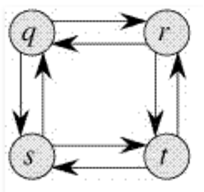
\includegraphics[width=0.2\textwidth]{Images/DPLongestPath}
\label{DPLongestPath}
\end{figure}

There are two longest paths from $q$ to $t$:
$q\to r\to t$ and $q\to s\to t$. Unlike shortest paths, these longest paths
do not have the optimal substructure property. For example, the longest path
$q\to r\to t$ is not a combination of longest path from $q$ to $r$ and
longest path from $r$ to $t$, because the longest path from $q$ to $r$ is
$q\to s\to t\to r$ and the longest path from $r$ to $t$ is $r\to q\to s\to
t$.

\section{How to solve a Dynamic Programming Problem?
  \label{secGFGDPHowToSolve}}

\textbf{Difficulty: 3.4}

\textbf{D}ynamic \textbf{P}rogramming (DP) is a technique that solves some
particular type of problems in \rrhl{Polynomial Time}. Dynamic Programming
solutions are faster than exponential brute method and can be easily proved
for their correctness.  Before we study how to think Dynamically for a
problem, we need to learn:
\begin{enumerate}[label=\textbf{\arabic*.}]
\item Overlapping Subproblems
\item Optimal Substructure Property
\end{enumerate}

\textbf{Steps to solve a DP}
\begin{enumerate}[label=\textbf{\arabic*.}]
\item Identify if it is a DP problem
\item Decide a state expression with least parameters
\item Formulate state relationship    
\item Do tabulation (or add memoization)
\end{enumerate}

\rrheader{Step 1 : How to classify a problem as a Dynamic Programming
  Problem?}

\begin{itemize}%[noitemsep,topsep=0pt]
\item Typically, \rrhl{all the problems that require to maximize or minimize
    certain quantity or counting problems that say to count the arrangements
    under certain condition or certain probability problems can be solved by
    using Dynamic Programming.}
\item \rrhl{All dynamic programming problems} satisfy the \rrhl{overlapping
    subproblems property} and \rrhl{most of the classic dynamic problems}
  also satisfy the \rrhl{optimal substructure property}. Once, we observe
  these properties in a given problem, be sure that it can be solved using
  DP.
\end{itemize}

\rrheader{Step 2 : Deciding the state}

DP problems are all about state and their transition. This is the most basic
step which must be done very carefully because the state transition depends
on the choice of state definition you make. So, let's see what do we mean by
the term ``state''.

\rrhl{State:} A state can be defined as the set of parameters that can
uniquely identify a certain position or standing in the given problem. This
set of parameters should be as small as possible to reduce state space.

For example: In our famous Knapsack
problem\footnote{\url{http://www.geeksforgeeks.org/knapsack-problem/}}, we
define our state by two parameters \textbf{index} and \textbf{weight} i.e
\ctt{DP[index][weight]}.  Here \ctt{DP[index][weight]} tells us the maximum
profit it can make by taking items from range $0$ to $index$ having the
capacity of sack to be weight.  Therefore, here the parameters index and
weight together can uniquely identify a subproblem for the knapsack problem.

So, our first step will be deciding a state for the problem after
identifying that the problem is a DP problem.

As we know DP is all about using calculated results to formulate the final
result.

So, our next step will be to find a relation between previous states to
reach the current state.

\rrheader{Step 3 : Formulating a relation among the states}

This part is the hardest part of for solving a DP problem and requires a
lots of intuition, observation and practice. Let's understand it by
considering a sample problem

\begin{mdframed}[style=mdfNOTE]

Given $3$ numbers $\brce*{1,3,5}$, we need to tell the total number of ways
we can form a number '$N$' using the sum of the given three numbers.
(allowing repetitions and different arrangements).

Total number of ways to form $6$ is : $8$\\
$1+1+1+1+1+1$\\
$1+1+1+3$\\
$1+1+3+1$\\
$1+3+1+1$\\
$3+1+1+1$\\
$3+3$\\
$1+5$\\
$5+1$\\

\end{mdframed}

Let's think dynamically for this problem. So, first of all, we decide a
state for the given problem. We will take a parameter $n$ to decide state as
it can uniquely identify any subproblem. So, our state dp will look like
state($n$). Here, state($n$) means the total number of arrangements to form
n by using $\brce*{1,3,5}$ as elements.

Now, we need to compute state($n$).

\rrheader{How to do it?}

So here the intuition comes into action. As we can only use $1$, $3$ or $5$
to form a given number. Let us assume that we know the result for
$n=1,2,3,4,5,6$; being termilogistic let us say we know the result for the
state($n=1$), state($n=2$), state($n=3$)$, \ldots, $ state($n=6$).

Now, we wish to know the result of the state($n=7$). See, we can only add
$1$, $3$ and $5$. Now we can get a sum total of $7$ by the following 3 ways:

\textbf{1) Adding 1 to all possible combinations of state($\textbf{n=6}$)}
E.g.:\\
$[ (1+1+1+1+1+1) + 1]$\\
$[ (1+1+1+3) + 1]$\\
$[ (1+1+3+1) + 1]$\\
$[ (1+3+1+1) + 1]$\\
$[ (3+1+1+1) + 1]$\\
$[ (3+3) + 1]$\\
$[ (1+5) + 1]$\\
$[ (5+1) + 1]$\\

\textbf{2) Adding 3 to all possible combinations of state($\bm{n=4}$)}

E.g.:\\
$[(1+1+1+1) + 3]$\\
$[(1+3) + 3]$\\
$[(3+1) + 3]$\\

\textbf{3) Adding 5 to all possible combinations of state($\bm{n=2}$)}

E.g.:\\
$[ (1+1) + 5]$

Now, think carefully and satisfy yourself that the above three cases are
covering all possible ways to form a sum total of $7$. \rrblue{(Yup, it's
  exhaustive.)}

Therefore, we can say that result for\\
state($7$) = state($6$) + state($4$) + state($2$)\\
or\\
state($7$) = state($7-1$) + state($7-3$) + state($7-5$)

In general,\\
\textbf{state($\bm{n}$) = state($\bm{n-1}$) + state($\bm{n-3}$) +
  state($\bm{n-5}$)}\\

So, our code will look like:
\begin{lstlisting}[style=raycppnewsnippet]
// Returns the number of arrangements to 
// form 'n' 
int solve(int n)
{ 
  // base case
  if (n < 0) 
    return 0;
  if (n == 0)  
    return 1;  
 
  return solve(n-1) + solve(n-3) + solve(n-5);
} 
\end{lstlisting}
The above code seems exponential as it is calculating the same state again
and again. So, we just need to add a memoization.

\rrheader{Step 4 : Adding memoization or tabulation for the state}

This is the easiest part of a dynamic programming solution. We just need to
store the state answer so that next time that state is required, we can
directly use it from our memory

Adding memoization to the above code
\begin{lstlisting}[style=raycppnewsnippet]
// initialize to -1
int dp[MAXN];
 
// this function returns the number of 
// arrangements to form 'n' 
int solve(int n)
{ 
  // base case
  if (n < 0)  
    return 0;
  if (n == 0)  
    return 1;
 
  // checking if already calculated
  if (dp[n]!=-1) 
      return dp[n];
 
  // storing the result and returning
  return dp[n] = solve(n-1) + solve(n-3) + solve(n-5);
}
\end{lstlisting}

Another way is to add tabulation and make solution iterative. Please refer
tabulation and
memoization\footnote{\url{http://www.geeksforgeeks.org/tabulation-vs-memoizatation/}}
for more details.

Dynamic Programming comes with a lots of practice. One must try solving
various classic DP problems that can be found
here\footnote{\url{http://www.geeksforgeeks.org/fundamentals-of-algorithms/#DynamicProgramming}}.
You may check the below problems first and try solving them using the above
described steps:-
\begin{itemize}%[noitemsep,topsep=0pt]
\item \url{http://www.spoj.com/problems/COINS/}
\item \url{http://www.spoj.com/problems/ACODE/}
\item
  \url{http://www.geeksforgeeks.org/dynamic-programming-set-6-min-cost-path/}
\item 
  \url{http://www.geeksforgeeks.org/dynamic-programming-subset-sum-problem/}
\item
  \url{http://www.geeksforgeeks.org/dynamic-programming-set-7-coin-change/}
\item
  \url{http://www.geeksforgeeks.org/dynamic-programming-set-5-edit-distance/}
\end{itemize}


%%%%%%%%%%%%%%%%%%%%%%%%%%%%%%%%%%%%%%%%%%%%%%%%%%%%%%%%%%%%%%%%%%%%%%%%%%%%
%%%%%%%%%%%%%%%%%%%%%%%%%%%%%%%%%%%%%%%%%%%%%%%%%%%%%%%%%%%%%%%%%%%%%%%%%%%%
%%%%%%%%%%%%%%%%%%%%%%%%%%%%%%%%%%%%%%%%%%%%%%%%%%%%%%%%%%%%%%%%%%%%%%%%%%%%

\section{Tabulation vs Memoizatation
  \label{secGFGDPTabVsMemo}}

\textbf{Difficulty: 2.7}

There are following two different ways to store the values so that the
values of a problem can be reused. Here, will discuss two patterns of
solving DP problem:
\begin{enumerate}[label=\textbf{\arabic*.}]
\item Tabulation: Bottom Up
\item Memoization: Top Down
\end{enumerate}
Before getting to the definitions of the above two terms consider the below
statements:
\begin{itemize}%[noitemsep,topsep=0pt]
\item \textbf{Version 1:} I will study the theory of Dynamic Programming
  from GeeksforGeeks, then I will practice some problems on classic DP and
  hence I will master Dynamic Programming.
\item \textbf{Version 2:} To Master Dynamic Programming, I would have to
  practice Dynamic problems and to practice problems---Firstly, I would have
  to study some theory of Dynamic Programming from GeeksforGeeks
\end{itemize}
Both the above versions say the same thing, just the difference lies in the
way of conveying the message and that's exactly what Bottom Up and Top Down
DP do. \textbf{Version 1} can be related to as Bottom Up DP and
\textbf{Version 2} can be related as Top Down DP.

\rrheader{Tabulation Method---Bottom Up Dynamic Programming}

As the name itself suggests starting from the bottom and cumulating answers
to the top. Let's discuss in terms of state transition.

Let's describe a state for our DP problem to be $dp[x]$ with $dp[0]$ as
base state and $dp[n]$ as our destination state. So, we need to find the
value of destination state i.e $dp[n]$.

If we start our transition from our base state i.e $dp[0]$ and follow our
state transition relation to reach our destination state $dp[n]$, we call it
\textbf{Bottom Up approach} as it is quite clear that we started our
transition from the bottom base state and reached the top most desired
state.

\rrheader{Now, Why do we call it tabulation method?}

To know this, let's first write some code to calculate the factorial of a
number using bottom up approach. Once, again as our general procedure to
solve a DP, we first define a state. In this case, we define a state as
$dp[x]$, where $dp[x]$ is to find  the factorial of $x$.

Now, it is quite obvious that $dp[x+1] = dp[x]\times (x+1)$
\begin{lstlisting}[style=raycppnewsnippet]
// Tabulated version to find factorial x.
int dp[MAXN];

// base case
int dp[0] = 1; // 0! = 1
for (int i = 1; i<=n; i++)
{
  dp[i] = dp[i-1] * i;
}
\end{lstlisting}
The above code clearly follows the bottom up approach as it starts its
transition from the bottom most base case $dp[0]$ and reaches it destination
state $dp[n]$. Here, we may notice that the $dp$ table is being populated
sequentially and we are \textbf{directly accessing the calculated states
  from the table itself} and hence, we call it tabulation method.

\rrheader{Memoization Method---Top Down Dynamic Programming}

Once, again let's describe it in terms of state transition. If we need to
find the value for some state say $dp[n]$ and instead of starting from the
base state, i.e. $dp[0]$, we ask our answer from the states that can be
reached from the destination state $dp[n]$, following the state transition
relation, then it is the top-down fashion of DP.

Here, we start our journey from the top most destination state and compute
its answer by taking in count the values of states that can reach the
destination state, till we reach the bottom most base state.

Once again, let's write the code for the factorial problem in top down
fashion
\begin{lstlisting}[style=raycppnewsnippet]
// Memoized version to find factorial x.
// To speed up we store the values
// of calculated states

// initialized to -1
int dp[MAXN]

// return fact x!
int solve(int x)
{
    if (x==0)
        return 1;
    if (dp[x]!=-1)
        return dp[x];
    return (dp[x] = x * solve(x-1));
}
\end{lstlisting}
As we can see we are storing the most recent cache up to a limit so that if
next time we got a call for the same state we simply return it from the
memory. So, this is why we call it memoization as we are storing the most
recent state values.

In this case the memory layout is linear that's why it may seem that the
memory is being filled in a sequential manner like the tabulation method,
but you may consider any other top down DP having 2D memory layout like Min
Cost
Path\footnote{http://www.geeksforgeeks.org/dynamic-programming-set-6-min-cost-path/},
here the memory is not filled in a sequential manner.

\begingroup
\renewcommand*{\arraystretch}{\arraystretchsize}
\begin{footnotesize}
\begin{longtable}{|p{2.5cm}|p{5.5cm}|p{5.5cm}|}
% header and footer information
\hline
\endfirsthead
\hline
\endlastfoot
% body of table
    &\textbf{Tabulation}&\textbf{Memoization}\\\hline
\textbf{State}&State Transition relation is difficult to think&State
transition relation is easy to think\\\hline
\textbf{Code} &Code gets complicated when lot of conditions are
required&Code is easy and less complicated\\\hline
\textbf{Speed}&Fast, as we directly access previous states from the
table&Slow due to a lot of recursive calls and return statements\\\hline
\textbf{Subproblem solving}&If all subproblems must be solved at least once,
bottom-up dynamic-programming algorithm usually outperforms a top-down
memoized algorithm by a constant factor.&If \textbf{\emph{some}} subproblem
in the subproblem space need not be solved at all, the memoized solution has
the advantage of solving only those subproblems that are definitely
required\\\hline
\textbf{Table Entries}&In the tabulated version, starting from the first
entry, all entries are filled on by one.& Unlike the tabulated version, all
entries of the lookup table re not necessarily filled in memoized version.
The table is filled on demand.
\end{longtable}
\end{footnotesize}
\endgroup


%%%%%%%%%%%%%%%%%%%%%%%%%%%%%%%%%%%%%%%%%%%%%%%%%%%%%%%%%%%%%%%%%%%%%%%%%%%%
%%%%%%%%%%%%%%%%%%%%%%%%%%%%%%%%%%%%%%%%%%%%%%%%%%%%%%%%%%%%%%%%%%%%%%%%%%%%
%%%%%%%%%%%%%%%%%%%%%%%%%%%%%%%%%%%%%%%%%%%%%%%%%%%%%%%%%%%%%%%%%%%%%%%%%%%%

\section{Dynamic Programming | Set 3 (Longest Increasing Subsequence)
  \label{secGFGDPSet3LIS}}

\url{http://www.geeksforgeeks.org/longest-increasing-subsequence/}

\textbf{Difficulty: 3.1}

Let us discuss Longest Increasing Subsequence (LIS) problem as an example
problem that can be solved using Dynamic Programming.

The Longest Increasing Subsequence (LIS) problem is to find the length of
the longest subsequence of a given sequence such that all elements of the
subsequence are sorted in increasing order. For example, the length of LIS
for $\brce*{10, 22, 9, 33, 21, 50, 41, 60, 80}$ is $6$ and LIS is
$\brce*{10, 22, 33, 50, 60, 80}$.

\begin{center}
\begin{tabular}{|c|c|c|c|c|c|c|c|c|c|}
\hline
\ctt{arr[]}&10&22&9&33&21&50&41&60&80\\\hline
LIS&1&2& &3& &4& &5&6\\ 
\hline
\end{tabular}
\end{center}

\begin{mdframed}[style=mdfNOTE,
frametitle={More examples}]

\begin{lstlisting}[style=raygeneric]
Input  : arr[] = {3, 10, 2, 1, 20}
Output : Length of LIS = 3
The longest increasing subsequence is 3, 10, 20

Input  : arr[] = {3, 2}
Output : Length of LIS = 1
The longest increasing subsequences are {3} and {2}

Input  : arr[] = {50, 3, 10, 7, 40, 80}
Output : Length of LIS = 4
The longest increasing subsequence is {3, 7, 40, 80}
\end{lstlisting}

\end{mdframed}

\RayNotesBegin

Oh, this was the longest increasing subsequence of the ``elementary''
section earlier. This is so much clearer with more examples.

Let's try to remember what we have to do:
\begin{enumerate}[label=\textbf{\arabic*.}]
\item \textbf{Identify if it is a DP problem:} For this to be a DP problem,
  \textbf{(1)} we need to identify a recursive solution which exhibits
  optimal substructure, by this I mean that the optimal solution is formed
  by optimal solutions to subproblems. \textbf{(2)} We also need overlapping
  subproblems. This is normally done by constructing the recursion tree for
  a particular set of input and seeing if there are repeated subproblems.
\item \textbf{Decide on a state expression with least parameters:} The state
  can be \textsc{lis}$[i]$, which is the longest increasing subsequence
  ending at $i$. E.g.

\begin{tabular}{|c|c|c|c|c|c|c|}
\hline
\ctt{arr[]}&8&9&6&7&4&5\\\hline
\ctt{lis[]}&1&2&1&2&1&2\\ 
\hline
\end{tabular}

\noindent{}Output : Length of $\textsc{lis}=2$\\
The longst incr. subseq. is: 8, 9 (select first one)\\
\textit{How did I get the \ctt{lis[]} values? Work through the \ctt{arr[]}
  values and for each one, count the length of the longest increasing
  subsequence ending \textbf{here}. So for $8$, clearly the \textsc{lis} is
  $1$. Next look at $9$, clearly the \textsc{lis} ending there is $2$. For
  $6$, there are no previous values in \ctt{arr} that can contribute to the
  \textsc{lis} ending here, so it's $\textsc{lis}=1$.}\\

\begin{tabular}{|c|c|c|c|c|c|c|}
\hline
\ctt{arr[]}&4&5&9&8&6&7\\\hline
\ctt{lis[]}&1&2&3&3&3&4\\ 
\hline
\end{tabular}

\noindent{}Output : Length of $\textsc{lis}=4$\\
The longst incr. subseq. is: $\brce*{4,5,6,7}$\\

\begin{tabular}{|c|c|c|c|c|c|c|c|c|c|}
\hline
\ctt{arr[]}&10&22&9&33&21&50&41&60&80\\\hline
\ctt{lis[]}& 1& 2&1& 3& 2& 4& 4& 5& 6\\ 
\hline
\end{tabular}

\noindent{}Output : Length of $\textsc{lis}=6$\\
The longst incr. subseq. is: $\brce*{10,22,33,50 (41),60,80}$\\

\begin{tabular}{|c|c|c|c|c|c|c|c|c|c|}
\hline
\ctt{arr[]}&3&10&2&1&20\\\hline
\ctt{lis[]}&1& 2&1&1&3\\ 
\hline
\end{tabular}

\noindent{}Output : Length of $\textsc{lis}=3$\\
The longst incr. subseq. is: $\brce*{3,10,20}$\\

\begin{tabular}{|c|c|c|c|c|c|c|c|c|c|}
\hline
\ctt{arr[]}&3&2\\\hline
\ctt{lis[]}&1&1\\ 
\hline
\end{tabular}

\noindent{}Output : Length of $\textsc{lis}=1$\\
The longst incr. subseqs. are: $\brce*{3}$ and $\brce*{2}$\\

\begin{tabular}{|c|c|c|c|c|c|c|c|c|c|}
\hline
\ctt{arr[]}&50&3&10&7&40&80\\\hline
\ctt{lis[]}& 1&1& 2&2& 3&4\\ 
\hline
\end{tabular}

\noindent{}Output : Length of $\textsc{lis}=4$\\
The longst incr. subseq. is: $\brce*{3,7,40,80}$\\

\item \textbf{Formulate state relationship:} Now that we have a state, think
  of how can we obtain a current state with previous states? Let's assume
  that the subsequence must be \emph{strictly increasing}. For convenience,
  let us rename \ctt{arr[]} to \ctt{A[]}. With this
  assumption (that the subsequence must be strictly increasing), we know 
  that \ctt{A[i]} is in a subsequence if and only if \ctt{A[i]} is greater
  than all other values in the subsequence. E.g. consider
\begin{tabular}{|c|c|c|c|c|c|c|c|c|c|}
\hline
\ctt{A[]}&10&20&30&25\\
\hline
\end{tabular},
 then $A[3]=25$ is in the LIS of $\brce*{10,20,25}$ since $25$ is greater
 than all over $A[j], j<i$, but $A[3]=25$ is not in the LIS of
 $\brce*{10,20,30,25}$, since $A[2] = 30 > A[3] = 25$. Thus, this is our
 first condition, we try to add $A[i]$ onto \textbf{\emph{each}} of the LIS
 ending with $A[j]$, $j<i$, such that $A[j]<A[i]$ (since this is the
 condition we stated above which guarantees a strictly increasing
 subsequence) and we choose the max length of this. E.g.
\begin{lstlisting}[style=raygeneric]
A[]={1,5,3,4,5}, consider A[3]=4, to see how this works, we write out the 
                 LIS ending at each A[j], j<i=3:
A[j=0] = {1},  yes since A[0]=1 <  A[3]=4
A[j=1] = {1,5} no  since A[1]=5 >= A[3]=4
A[j=2] = {1,3} yes since A[2]=3 <  A[3]=4
\end{lstlisting}
Now we choose the max length out of all the possible ones, and record that
in $lis[i]$, in this case it happens to be $\brce*{1,3,4}$ of length $3$. We
formalise this with the recurrent relation:
\begin{equation*}
\textsc{lis}[i]=\max_{j<i}\set*{L[j] \given A[j]<A[i]}
\end{equation*}

Initial/boundary conditions: We start from the left of $A[]$ and build up
$lis[]$ in the same manner. Thus the initial condition is
\begin{equation*}
lis[0]=1
\end{equation*}
since the LIS ending at $A[0]$ has length $1$ (in other words, the element
in $A[0]$).

\item Do tabulation (or add memoization): we'll do tabulation, since it
  seems like we'll need to work out the \textsc{lis} for all entries.
\end{enumerate}

Okay, let's try code this up!  Code found in:\\
\path{src/DynamicProgramming/rrrGFGDPSet3LIS.cpp}
\begin{lstlisting}[style=raycppnewsnippet]
template<typename T>
auto longestIncreSubseq(const vector<T>& A)
{
  using vecSz_t = decltype(A.size());
  auto n = A.size();

  vector<T> lis(n,0);
  
  // base case: lis of first number is 1
  lis[0] = 1;

  // Loop for lis[i], i=1..n-1
  for(vecSz_t i = 1; i < n; ++i)
  {
    // There is always a LIS of length at least 1 ending in A[i] 
    // (the element already in there!)
    lis[i] = 1;
    // Consider each previous lis[j], j<i
    for(vecSz_t j = 0; j<i; ++j)
    {
      // We need to plus one to account for the element ending at A[i].
      // So if lis[j]+A[i] is a valid subsequence (A[j]<A[i]),
      // then it must be of length lis[j]+1, we compare if this is greater
      // than what's currently calculated for lis[i].
      if((lis[j]+1)>lis[i] && A[j]<A[i])
      {
        lis[i] = lis[j]+1;
      }
    }
  }

  return lis;
}

int main()
{
  auto lis = longestIncreSubseq<int>({50,3,10,7,40,80});
  printSeqCon(lis, "lis: ");
  return 0;
}
\end{lstlisting}
I'm not sure if I have to do tabulation, I think I've done it already. Now
onto read the GFG solution.

\RayNotesEnd

\rrheader{Optimal substructure:}

Let \ctt{arr[0..n-1]} be the input array and \ctt{L(i)} be the length of the
LIS \textbf{ending at index $\bm{i}$} such that \ctt{arr[i]} is the last
element of the LIS.\\

Then, $L(i)$ can be recursively written as:\\ 
$L(i) = 1 + max( L(j) )$ where $0 < j < i$ and $arr[j] < arr[i]$; or\\ 
$L(i) = 1$, if no such $j$ exists.\\

To find the LIS for a given array, we need to return $\max(L(i))$ where
$0<i<n$. Thus, we see the LIS problem satisfies the optimal substructure
property \rrhl{as the main problem can be solved using solutions to
  subproblems}.

Following is a simple recursive implementation of the LIS problem. It
follows the recursive structure discussed above.
\begin{lstlisting}[style=raycppnewsnippet]
/* A Naive C/C++ recursive implementation of LIS problem */
#include<stdio.h>
#include<stdlib.h>
 
/* To make use of recursive calls, this function must return
   two things:
   1) Length of LIS ending with element arr[n-1]. We use
      max_ending_here for this purpose
   2) Overall maximum as the LIS may end with an element
      before arr[n-1], max_ref is used this purpose.

   The value of LIS of full array of size n is stored in
   *max_ref which is our final result */
int _lis( int arr[], int n, int *max_ref)
{
  /* Base case */
  if (n == 1)
    return 1;
 
  // 'max_ending_here' is length of LIS ending with arr[n-1]
  int res, max_ending_here = 1; 
 
  /* Recursively get all LIS ending with arr[0], arr[1] ...
     arr[n-2]. If arr[i-1] is smaller than arr[n-1], and
     max ending with arr[n-1] needs to be updated, then
     update it */
  for (int i = 1; i < n; i++)
  {
    res = _lis(arr, i, max_ref);
    if (arr[i-1] < arr[n-1] && res + 1 > max_ending_here)
      max_ending_here = res + 1;
  }
 
  // Compare max_ending_here with the overall max. And
  // update the overall max if needed
  if (*max_ref < max_ending_here)
    *max_ref = max_ending_here;
 
  // Return length of LIS ending with arr[n-1]
  return max_ending_here;
}

// The wrapper function for _lis()
int lis(int arr[], int n)
{
  // The max variable holds the result
  int max = 1;
 
  // The function _lis() stores its result in max
  _lis( arr, n, &max );
 
  // returns max
  return max;
}
 
/* Driver program to test above function */
int main()
{
  int arr[] = { 10, 22, 9, 33, 21, 50, 41, 60 };
  int n = sizeof(arr)/sizeof(arr[0]);
  printf("Length of lis is %dn",
         lis( arr, n ));
  return 0;
}
\end{lstlisting}
Output:
\begin{lstlisting}[style=rayio]
Length of lis is 5
\end{lstlisting}

\rrheader{Overlapping Subproblems:}

Considering the above implementation, following is recursion tree for an
array of size $4$. \ctt{lis(n)} gives us the length of LIS for \ctt{arr[]}.
\begin{lstlisting}[style=pseudostyle]
              lis(4)
        /        |     
      lis(3)    lis(2)   lis(1)
     /           /
   lis(2) lis(1) lis(1)
   /
lis(1)
\end{lstlisting}
We can see that there are many subproblems which are solved again and again.
So this problem has Overlapping Substructure property and recomputation of
same subproblems can be avoided by either using Memoization or Tabulation.
Following is a tabluated implementation for the LIS problem.
\begin{lstlisting}[style=raycppnewsnippet]
/* Dynamic Programming C/C++ implementation of LIS problem */
#include<stdio.h>
#include<stdlib.h>
 
/* lis() returns the length of the longest increasing
  subsequence in arr[] of size n */
int lis( int arr[], int n )
{
  int *lis, i, j, max = 0;
  lis = (int*) malloc ( sizeof( int ) * n );
 
  /* Initialize LIS values for all indexes */
  for (i = 0; i < n; i++ )
    lis[i] = 1;
 
  /* Compute optimized LIS values in bottom up manner */
  for (i = 1; i < n; i++ )
    for (j = 0; j < i; j++ ) 
      if ( arr[i] > arr[j] && lis[i] < lis[j] + 1)
        lis[i] = lis[j] + 1;
 
    /* Pick maximum of all LIS values */
    for (i = 0; i < n; i++ )
      if (max < lis[i])
        max = lis[i];
 
    /* Free memory to avoid memory leak */
    free(lis);
 
    return max;
}
/* Driver program to test above function */
int main()
{
  int arr[] = { 10, 22, 9, 33, 21, 50, 41, 60 };
  int n = sizeof(arr)/sizeof(arr[0]);
  printf("Length of lis is %dn", lis( arr, n ) );
  return 0;
}
\end{lstlisting}

Output:
\begin{lstlisting}[style=rayio]
Length of lis is 5
\end{lstlisting}
Note that the time complexity of the above Dynamic Programming (DP) solution
is $\comBigOh{n^2}$ and there is a $\comBigOh{n\log n}$ solution for the LIS
problem. We have not discussed the $\comBigOh{n\log n}$ solution here as the
purpose of this post is to explain Dynamic Programming with a simple
example. See below post for $\comBigOh{n\log n}$ solution.

\RayNotesBegin

RRRTODO - check this out:
\url{http://www.geeksforgeeks.org/longest-increasing-subarray/}

The $\comBigOh{n\log n}$ solution is here: \url{http://www.geeksforgeeks.org/longest-monotonically-increasing-subsequence-size-n-log-n/}

\RayNotesEnd

%%%%%%%%%%%%%%%%%%%%%%%%%%%%%%%%%%%%%%%%%%%%%%%%%%%%%%%%%%%%%%%%%%%%%%%%%%%%
%%%%%%%%%%%%%%%%%%%%%%%%%%%%%%%%%%%%%%%%%%%%%%%%%%%%%%%%%%%%%%%%%%%%%%%%%%%%
%%%%%%%%%%%%%%%%%%%%%%%%%%%%%%%%%%%%%%%%%%%%%%%%%%%%%%%%%%%%%%%%%%%%%%%%%%%%

\section{Dynamic Programming | Set 4 (Longest Common Subsequence)
  \label{secGFGDPSet4LCS}}

\url{http://www.geeksforgeeks.org/longest-common-subsequence}

\textbf{Difficulty: 2.8}

We have discussed Overlapping Subproblems and Optimal Substructure
properties in Set 1 (\pagecref{secGFGDPSet1OverlapSubprob}) and Set 2
(\pagecref{secGFGDPSet2OptimalSubstruct}) respectively. We also discussed
one example problem in Set 3 (\pagecref{secGFGDPSet3LIS}). Let us discuss
Longest Common Subsequence (LCS) problem as one more example problem that
can be solved using Dynamic Programming.

\begin{quotation}
\textbf{LCS Problem Statement:} Given two sequences, find the length of
longest subsequence present in both of them. A subsequence is a sequence
that appears in the \textbf{same relative order}, but \rrhl{not necessarily
  contiguous}. For example, ``abc'', ``abg'', ``bdf'', ``aeg'', ``acefg'',
.. etc are subsequences of ``abcdefg''. So a string of length $n$ has $2^n$
different possible subsequences \rrblue{(since a character is either present
  or it isn't)}.
\end{quotation}

It is a classic computer science problem, the basis of diff (a file
comparison program that outputs the differences between two files), and has
applications in bioinformatics.

Examples:
\begin{itemize}%[noitemsep,topsep=0pt]
\item LCS for input Sequences ``ABCDGH'' and ``AEDFHR'' is ``ADH'' of length
  3.
\item LCS for input Sequences ``AGGTAB'' and ``GXTXAYB'' is ``GTAB'' of
  length 4.
\end{itemize}

\textbf{\rrgreen{Recommended: Please solve it on ``PRACTICE'' first, before
    moving on to the solution.}}

\RayNotesBegin

Let's try to remember what we have to do:
\begin{enumerate}[label=\textbf{\arabic*.}]
\item Identify if it is a DP problem: I.e. do we have an optimal
  substructure and overlapping subproblems?
\item Decide on a state expression with least parameters: What parameters
  describe the problem/solution?
\item Formulate state relationship: Say if we have the solution for $i$, we
  have to put it in terms of the solutions previous to $i$.
\item Do tabulation (or add memoization): Choose one!
\end{enumerate}

Items (1)-(3) seems like they can be done together. We need a bit of
intuition. 
\begin{itemize}%[noitemsep,topsep=0pt]
\item First think, we're trying to find the LCS of two sequences $X[0..m-1]$
  and $Y[0..n-1]$. Assume we already have this LSC, call it $Z[0..k-1]$. So
  I guess we can express the \textbf{state} as 
\begin{equation*}
Z[0..k-1] = \textsc{LCS}(X[0..m-1],Y[0..n-1]) 
\end{equation*}
\item Now we need formulate the state relationship. I.e. express $Z[0..k-1]$
  in terms of previous $Z[0..k-j]$, where $1<j\leq k$. To do this, look at
  what we know, we know that $Z[0..k-1]$ is the LCS of $X[0..m-1]$ and
  $Y[0..n-1]$, this implies that $Z[0..k-1]$ contains characters common to
  both $X[0..m-1]$ and $Y[0..n-1]$ \textbf{\emph{This is the insight we
      needed to make the leap to an optimal substructure}}.
  \textbf{\emph{This is where intuition kicks in:}} 

  Working from the end of the lists (so we're going from right to left), we
  compare $X[m-1]$ and $Y[n-1]$, there are three possibilities:
  
  \begin{enumerate}[label=\textbf{\arabic*.}]
  \item $X[m-1] == Y[n-1]$ implies that $Z[k-1] == X[m-1] == Y[n-1]$, so 
  \begin{equation*}
    Z[0..k-1] = Z[k-1] + \textsc{LCS}(X[0..m-2],Y[0..n-2])
  \end{equation*}
  \item $X[m-1] \neq Y[n-1]$ and $Z[k-1] == X[m-1]$ implies that 
  \begin{equation*}
    Z[0..k-1] = \textsc{LCS}(X[0..m-1],Y[0..n-2])
  \end{equation*}
  \item $X[m-1] \neq Y[n-1]$ and $Z[k-1] == Y[n-1]$ implies that 
  \begin{equation*}
    Z[0..k-1] = \textsc{LCS}(X[0..m-2],Y[0..n-1])
  \end{equation*}
  \end{enumerate}
  Now for convenience, let $\textsc{LCS-L}(X[],Y[])$ be a function which
  returns the length of the LCS. We can now combine \textbf{(2)} and
  \textbf{(3)} to give the following recurrence relation:
  \begin{equation*}
\resizebox{0.91\hsize}{!}{%
  $
  \begin{split}
  &\textsc{LCS-L}(X[0..m-1],Y[0..n-1])=\\
  &\begin{cases}
  1+\textsc{LCS-L}(X[0..m-2],Y[0..n-2])&\text{ if $X[m-1] == Y[n-1]$,}\\
  \max(\textsc{LCS-L}(X[0..m-1],Y[0..n-2]),\textsc{LCS-L}(X[0..m-2],Y[0..n-1])) &\text{ otherwise.}
  \end{cases}
  \end{split}
  $}
  \end{equation*}

  \textbf{Quote from CLRS(p. 393):} Theorem 15.1 implies that we should
  examine either one or two subproblems when finding an LCS of
  $X_{m-1}=\braket*{x_0,\ldots,x_{m-1}}$ and
  $Y_{n-1}=\braket*{y_0,\ldots,y_{n-1}}$. If $x_{m-1}==y_{n-1}$, we must
  find an LCS of $X_{m-2}$ and $Y_{n-2}$.  Appending $x_{m-1}==y_{n-1}$ to
  this LCS yields an LCS of $X_{m-1}$ and $Y_{n-1}$. If $x_{m-1}\neq
  y_{n-1}$, then we must solve two subproblems: finding an LCS of $X_{m-2}$
  and $Y_{n-1}$ and finding an LCS of $X_{m-1}$ and $Y_{n-2}$.  Whichever of
  these two LCSs is longer is an LCS of $X_{m-1}$ and $Y_{n-1}$. Because
  these cases exhaust all possibilities, we know that one of the optimal
  subproblem solutions must appear within an LCS of $X_{m-1}$ and $Y_{n-1}$.

  We can readily see the overlapping-subproblems property in the LCS
  problem. To find an LCS of $X_{m-1}$ and $Y_{n-1}$, we may need to find
  the LCSs of $X_{m-1}$ and $Y_{n-2}$ and of $X_{m-2}$ and $Y_{n-1}$. But
  each of these subproblems has the subsubproblem of finding an LCS of
  $X_{m-2}$ and $Y_{n-2}$. Many other subproblems share subsubproblems.

  As in the matrix-chain multiplication problem, our recursive solution to
  the LCS problem involves establishing a recurrence for the value of an
  optimal solution. Let us define $c[i,j]$ to be the length of an LCS of the
  sequences $X_i$ and $Y_j$. If either $i=0$ or $j=0$, one of the sequences
  has length $0$, and so the LCS has length $0$. The optimal substructure of
  the LCS problem gives the recursive formula (size of $c$ is n+1)
  \begin{equation}\label{eqCLRSC15N9}
  c[i,j] = 
  \begin{cases}
  0            &\text{ if $i=0$ or $j=0$,}\\
  c[i-1,j-1]+1 &\text{ if $i,j>0$ and $x_i==y_j$,}\\
  \max(c[i,j-1],c[i-1,j]) &\text{ if $i,j>0$ and $x_i\neq y_j$.}
  \end{cases}
  \end{equation}
  
  Observe that in this recursive formulation, a condition in the problem
  restricts which subproblems we may consider. When $x_i=y_j$, we can and
  should consider the subproblem of finding an LCS of $X_{i-1}$ and
  $Y_{j-1}$.  Otherwise, we instead consider the two subproblems of finding
  an LCS of $X_i$ and $Y_{j-1}$ and of $X_{i-1}$ and $Y_j$. In the previous
  dynamic-programming algorithms we have examined---for rod cutting and
  matrix-chain multiplication---we ruled out no subproblems due to
  conditions in the problem. Finding an LCS is not the only
  dynamic-programming algorithm that rules out subproblems based on
  conditions in the problem.  For example, the edit-distance problem (see
  Problem 15-5) has this characteristic.

\item \textbf{Implementation:} Based on \cref{eqCLRSC15N9}, we could easily
  write an exponential-time recursive algorithm to compute the length of an
  LCS of two sequences. Since the LCS problem has only $\comTheta{mn}$
  distinct subproblems, however, we can use dynamic programming to compute
  the solutions bottom up.

  Procedure \textsc{LCS-Length} takes two sequences
  $X_{n-1}=\braket*{x_0,x_1,\ldots,x_{m-1}}$ and
  $Y_{m-1}=\braket*{y_0,y_1,\ldots,y_{n-1}}$ as inputs. It stores the
  $c[i,j]$ values in a table $c[0..m,0..n]$, and it computes the entries in
  \textbf{row-major} order. (That is, the procedure fills in the first row
  of $c$ from left to right, then the second row, and so on.). The procedure
  returns the table $c$; $c[m,n]$ contains the length of an LCS of $X_{m-1}$
  and $Y_{n-1}$.

\end{itemize}


Okay, let's try code this up!
Code found in:\\ 
\path{src/DynamicProgramming/rrrGFGLCS.cpp}

I've coded up both the recursive version without DP:
\begin{lstlisting}[style=raycppnewsnippet]
// Function to find the longest common subsequence of two strings X and Y.
// of length m and n, respectively. Thus, X[0..m] and Y[0..n].
// Returns the length of the longest common substring found. This does not
// use DP.
auto lcs_length_recur(const string& X, const string& Y, 
                      decltype(X.size()) m, decltype(Y.size()) n)
  ->common_type_t<decltype(X.size()),decltype(Y.size())>
{
  // base case, if m or n equals 0, then we have no characters in one of
  // the substrings, which implies that the longest common subsequence in
  // this case is 0.
  if(m==0 || n == 0)
  {
    return 0;
  }
  // X[m-1]==Y[n-1] implies that this character is a part of the LCS. Thus
  // we know the LCS contains this character plus the LCS of the lower state
  // for X and Y. Note the difference in indices between how we index the
  // substrings X and Y and what we pass to the lcs function. That is, when
  // we pass m and n to lcs, the characters we're looking at in X and Y are
  // m-1 and n-1, respectively. Thus, when we want the lower states, we pass
  // m-1 and n-1 to lcs, instead of m-2 and n-1. This is correct since m and
  // n describes the length of the substrings, whilst indexing is from base
  // 0.
  else if(X[m-1] == Y[n-1])
  {
    return 1+lcs_length_recur(X,Y,m-1,n-1);
  }
  // Otherwise X[m-1]!=Y[n-1] implies either X[m-1] does not contribute to
  // the lcs and lcs is in (X[m-2],Y[n-1]) or Y[n-1] does not contribute to
  // the lcs and lsc is in (X[m-1],Y[n-2]). We want the max of this.
  else
  {
    return max(lcs_length_recur(X,Y,m,n-1),
               lcs_length_recur(X,Y,m-1,n));
  }
}
\end{lstlisting}
With DP, bottom up with tabulation:
\begin{lstlisting}[style=raycppnewsnippet]
// LCS - DP with bottom up tabulation method.
// Returns the length of LCS.
auto lcs_length_tabulate(const string& X, const string& Y)
{
  using strsize_t = decltype(X.size());
  strsize_t m = X.size();
  strsize_t n = Y.size();

  vector<vector<int>>c(m+1,vector<int>(n+1,0));

  // Loop through the rows, starting from 1
  for(strsize_t i = 1; i != (m+1); ++i)
  {
    // Loop through the columns, starting from 1
    for(strsize_t j = 1; j != (n+1); ++j)
    {
      // These indices make sense, because range of X is X[0..n-1]
      // and i = 1..n.
      //
      // That is, c[i][j] contains the length of LCS of substrings of 
      // LENGTHS i and j. Indices of X and Y are: X[0..i-1] and Y[0..j-1].
      if(X[i-1] == Y[j-1])
        c[i][j] = c[i-1][j-1]+1;
      else
        c[i][j] = max(c[i-1][j], c[i][j-1]);
    }
  }
  return c[m][n];
}
\end{lstlisting}

\RayNotesEnd

\rrheader{\rrgreen{Now we continue with Geeksforgeeks solution}}

The naive solution for this problem is to generate all subsequences of both
given sequences and find the longest matching subsequence. This solution is
exponential in term of time complexity. Let us see how this problem
possesses both important properties of a Dynamic Programming (DP) Problem.

\rrheader{(1) Optimal Substructure:}

Let the input sequences be $X[0..m-1]$ and $Y[0..n-1]$ of lengths $m$ and
$n$ respectively. And let $L(X[0..m-1],Y[0..n-1])$ be the length of LCS of
the two sequences $X$ and $Y$. Following is the recursive definition of
$L(X[0..m-1],Y[0..n-1])$.
\begin{itemize}%[noitemsep,topsep=0pt]
\item If last characters of both sequences match (or $X[m-1]==Y[n-1]$) then
  $L(X[0..m-1],Y[0..n-1])=1+L(X[0..m-2],Y[0..n-2])$
\item If last characters of both sequences do not match (or
  $X[m-1]!=Y[n-1]$) then $L(X[0..m-1],Y[0..n-1])=$\\
  $MAX(L(X[0..m-2],Y[0..n-1]),L(X[0..m-1],Y[0..n-2])$
\end{itemize}

\rrheader{Examples:}

\begin{enumerate}[label=\textbf{\arabic*.}]
\item Consider the input strings ``AGGTAB'' and ``GXTXAYB''. Last characters
match for the strings. So length of LCS can be written as:\\
$L(\text{``AGGTAB''},\text{``GXTXAYB''}) = 1 +
L(\text{``AGGTA''},\text{``GXTXAY''})$
\begin{figure}
\centering
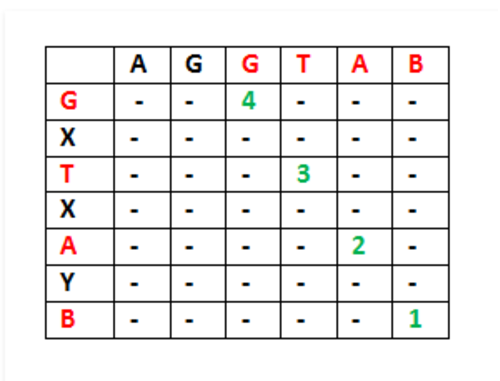
\includegraphics[width=0.5\textwidth]{Images/figGFGDPSet4LCS}
\label{figGFGDPSet4LCS}
\end{figure}
\item Consider the input strings ``ABCDGH'' and ``AEDFHR''. Last characters
  do not match for the strings. So length of LCS can be written as:\\
$L(\text{``ABCDGH''},\text{``AEDFHR''})=$\\
$MAX(L(\text{``ABCDG''},\text{``AEDFH\textbf{R}''}),L(\text{``ABCDG\textbf{H}''},\text{``AEDFH''}))$
\end{enumerate}

So the LCS problem has optimal substructure property as the main problem can
be solved using solutions to subproblems.

\rrheader{(2) Overlapping Subproblems:}

Following is simple recursive implementation of the LCS problem. The
implementation simply follows the recursive structure mentioned above.
\begin{lstlisting}[style=raycppnewsnippet]
/* A Naive recursive implementation of LCS problem */
#include<bits/stdc++.h>
 
int max(int a, int b);
 
/* Returns length of LCS for X[0..m-1], Y[0..n-1] */
int lcs( char *X, char *Y, int m, int n )
{
   if (m == 0 || n == 0)
     return 0;
   if (X[m-1] == Y[n-1])
     return 1 + lcs(X, Y, m-1, n-1);
   else
     return max(lcs(X, Y, m, n-1), lcs(X, Y, m-1, n));
}
 
/* Utility function to get max of 2 integers */
int max(int a, int b)
{
    return (a > b)? a : b;
}
 
/* Driver program to test above function */
int main()
{
  char X[] = "AGGTAB";
  char Y[] = "GXTXAYB";
 
  int m = strlen(X);
  int n = strlen(Y);
 
  printf("Length of LCS is %dn", lcs( X, Y, m, n ) );
 
  return 0;
}
\end{lstlisting}
Output:
\begin{lstlisting}[style=rayio]
Length of LCS is 4
\end{lstlisting}
Time complexity of the above naive recursive approach is $\comBigOh{(2^n)}$
in worst case and worst case happens when all characters of $X$ and $Y$
mismatch i.e., length of LCS is $0$.

Considering the above implementation, following is a partial recursion tree
for input strings ``AXYT'' and ``AYZX''
\begin{lstlisting}[style=pseudostyle]
                         lcs("AXYT", "AYZX")
                       /                 
         lcs("AXY", "AYZX")            lcs("AXYT", "AYZ")
         /                              /               
lcs("AX", "AYZX") lcs("AXY", "AYZ")   lcs("AXY", "AYZ") lcs("AXYT", "AY")
\end{lstlisting}
In the above partial recursion tree, $lcs(\text{``AXY''},\text{``AYZ''})$ is
being solved twice. If we draw the complete recursion tree, then we can see
that there are many subproblems which are solved again and again. So this
problem has Overlapping Substructure property and recomputation of same
subproblems can be avoided by either using Memoization or Tabulation.
Following is a tabulated implementation for the LCS problem.
\begin{lstlisting}[style=raycppnewsnippet]
/* Dynamic Programming C/C++ implementation of LCS problem */
#include<bits/stdc++.h>
  
int max(int a, int b);
  
/* Returns length of LCS for X[0..m-1], Y[0..n-1] */
int lcs( char *X, char *Y, int m, int n )
{
   int L[m+1][n+1];
   int i, j;
  
   /* Following steps build L[m+1][n+1] in bottom up fashion. Note 
      that L[i][j] contains length of LCS of X[0..i-1] and Y[0..j-1] */
   for (i=0; i<=m; i++)
   {
     for (j=0; j<=n; j++)
     {
       if (i == 0 || j == 0)
         L[i][j] = 0;
  
       else if (X[i-1] == Y[j-1])
         L[i][j] = L[i-1][j-1] + 1;
  
       else
         L[i][j] = max(L[i-1][j], L[i][j-1]);
     }
   }
    
   /* L[m][n] contains length of LCS for X[0..n-1] and Y[0..m-1] */
   return L[m][n];
}
/* Utility function to get max of 2 integers */
int max(int a, int b)
{
    return (a > b)? a : b;
}
  
/* Driver program to test above function */
int main()
{
  char X[] = "AGGTAB";
  char Y[] = "GXTXAYB";
  
  int m = strlen(X);
  int n = strlen(Y);
  
  printf("Length of LCS is %dn", lcs( X, Y, m, n ) );
 
  return 0;
}
\end{lstlisting}
Time Complexity of the above implementation is $\comBigOh{(mn)}$ which is
much better than the worst case time complexity of Naive Recursive
implementation.

The above algorithm/code returns only length of LCS. Please see the
following post for printing the LCS. Printing Longest Common Subsequence
(see \pagecref{secGFGDPLCSPrint})

You can also check the space optimized version of LCS at Space Optimized
Solution of LCS (see \pagecref{secGFGDPLCSSpaceOptimized})


%%%%%%%%%%%%%%%%%%%%%%%%%%%%%%%%%%%%%%%%%%%%%%%%%%%%%%%%%%%%%%%%%%%%%%%%%%%%
%%%%%%%%%%%%%%%%%%%%%%%%%%%%%%%%%%%%%%%%%%%%%%%%%%%%%%%%%%%%%%%%%%%%%%%%%%%%
%%%%%%%%%%%%%%%%%%%%%%%%%%%%%%%%%%%%%%%%%%%%%%%%%%%%%%%%%%%%%%%%%%%%%%%%%%%%

\subsection{Printing Longest Common Subsequence
  \label{secGFGDPLCSPrint}}

\url{http://www.geeksforgeeks.org/printing-longest-common-subsequence/}

\textbf{Difficulty: 3.2}

Given two sequences, print the longest subsequence present in both of them.

\rrheader{Examples:}
\begin{itemize}%[noitemsep,topsep=0pt]
\item LCS for input Sequences ``ABCDGH'' and ``AEDFHR'' is ``ADH'' of length
  3.
\item LCS for input Sequences ``AGGTAB'' and ``GXTXAYB'' is ``GTAB'' of
  length 4.
\end{itemize}

We have discussed Longest Common Subsequence (LCS) problem in a previous
post (see \pagecref{secGFGDPSet4LCS}). The function discussed there was
mainly to find the length of LCS. To find length of LCS, a 2D table $L[][]$
was constructed. In this post, the function to construct and print LCS is
discussed.

Following is detailed algorithm to print the LCS. It uses the same 2D table
$L[][]$.
\begin{enumerate}[label=\textbf{\arabic*.}]
\item Construct $L[m+1][n+1]$ using the steps discussed in previous post.
\item The value $L[m][n]$ contains length of LCS. Create a character array
  $lcs[]$ of length equal to the length of lcs plus 1 (one extra to store
  $\backslash0$ \rrblue{(\textsc{nil})}).
\item Traverse the 2D array starting from $L[m][n]$. Do following for every
  cell $L[i][j]$
  \begin{enumerate}[label=\textbf{\alph*.}]
  \item If characters (in X and Y) corresponding to $L[i][j]$ are same (Or
    $X[i-1] == Y[j-1]$), then include this character as part of LCS.
  \item Else compare values of $L[i-1][j]$ and $L[i][j-1]$ and go in
    direction of greater value.
  \end{enumerate}
\end{enumerate}

The following table (taken from
Wiki\footnote{\url{https://en.wikipedia.org/wiki/Longest\_common\_subsequence\_problem}})
shows steps (highlighted) followed by the above algorithm.

\begin{figure}
\centering
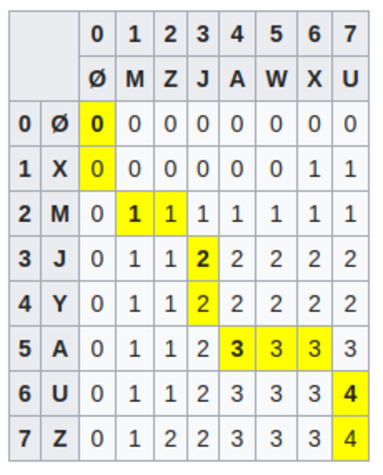
\includegraphics[width=0.4\textwidth]{Images/figGFGDPSet4LCSPrint}
\label{figGFGDPSet4LCSPrint}
\end{figure}

\textbf{\rrgreen{Recommended: Please try your approach first, before moving
    on to the solution.}}

\RayNotesBegin

This is in the same file as the lcs code:\\
\path{src/DynamicProgramming/rrrGFGLCS.cpp}
\begin{lstlisting}[style=raycppnewsnippet]
template<typename S, typename T>
auto get_lcs(S& str1, S& str2, T c)
{
  // store the lcs characters, note: since we are using arrays, we do not
  // need the terminating character.
  auto m = str1.size();
  auto n = str2.size();

  vector<std::remove_cv_t<std::remove_reference_t<decltype(str1[0])> > > 
    lcs_chars(c[m][n]);
  auto i = m;
  auto j = n;
  auto lcs_index = c[m][n];

  while(i>0 && j>0)
  {
    if(str1[i-1] == str2[j-1])
    {
      lcs_chars[lcs_index-1] = str1[i-1];
      --i; --j; --lcs_index;
    }
    // move up? Note that we do NOt minus one from c[][] indices. Since this
    // array contains 0 at the upper left.
    else if(c[i-1][j]>c[i][j-1])
      --i;
    // move to the left
    else 
      --j;
  }

  return lcs_chars;
}
\end{lstlisting}

\RayNotesEnd

Following is C++ implementation of above approach.
\begin{lstlisting}[style=raycppnewsnippet]
/* Dynamic Programming implementation of LCS problem */
#include<iostream>
#include<cstring>
#include<cstdlib>
using namespace std;
 
/* Returns length of LCS for X[0..m-1], Y[0..n-1] */
void lcs( char *X, char *Y, int m, int n )
{
   int L[m+1][n+1];
 
   /* Following steps build L[m+1][n+1] in bottom up fashion. Note
      that L[i][j] contains length of LCS of X[0..i-1] and Y[0..j-1] */
   for (int i=0; i<=m; i++)
   {
     for (int j=0; j<=n; j++)
     {
       if (i == 0 || j == 0)
         L[i][j] = 0;
       else if (X[i-1] == Y[j-1])
         L[i][j] = L[i-1][j-1] + 1;
       else
         L[i][j] = max(L[i-1][j], L[i][j-1]);
     }
   }
 
   // Following code is used to print LCS
   int index = L[m][n];
 
   // Create a character array to store the lcs string
   char lcs[index+1];
   lcs[index] = '\0'; // Set the terminating character
   
   // Start from the right-most-bottom-most corner and
   // one by one store characters in lcs[]
   int i = m, j = n;
   while (i > 0 && j > 0)
   {
      // If current character in X[] and Y are same, then
      // current character is part of LCS
      if (X[i-1] == Y[j-1])
      {
          lcs[index-1] = X[i-1]; // Put current character in result
          i--; j--; index--;     // reduce values of i, j and index
      }
 
      // If not same, then find the larger of two and
      // go in the direction of larger value
      else if (L[i-1][j] > L[i][j-1])
         i--;
      else
         j--;
   }
 
   // Print the lcs
   cout << "LCS of " << X << " and " << Y << " is " << lcs;
}
/* Driver program to test above function */
int main()
{
  char X[] = "AGGTAB";
  char Y[] = "GXTXAYB";
  int m = strlen(X);
  int n = strlen(Y);
  lcs(X, Y, m, n);
  return 0;
}
\end{lstlisting}
Output:
\begin{lstlisting}[style=rayio]
LCS of AGGTAB and GXTXAYB is GTAB
\end{lstlisting}

%%%%%%%%%%%%%%%%%%%%%%%%%%%%%%%%%%%%%%%%%%%%%%%%%%%%%%%%%%%%%%%%%%%%%%%%%%%%
%%%%%%%%%%%%%%%%%%%%%%%%%%%%%%%%%%%%%%%%%%%%%%%%%%%%%%%%%%%%%%%%%%%%%%%%%%%%
%%%%%%%%%%%%%%%%%%%%%%%%%%%%%%%%%%%%%%%%%%%%%%%%%%%%%%%%%%%%%%%%%%%%%%%%%%%%

\subsection{A Space Optimized Solution of LCS
  \label{secGFGDPLCSSpaceOptimized}}

\url{http://www.geeksforgeeks.org/space-optimized-solution-lcs}

\textbf{Difficulty: 2.5}

TODO

%%%%%%%%%%%%%%%%%%%%%%%%%%%%%%%%%%%%%%%%%%%%%%%%%%%%%%%%%%%%%%%%%%%%%%%%%%%%
%%%%%%%%%%%%%%%%%%%%%%%%%%%%%%%%%%%%%%%%%%%%%%%%%%%%%%%%%%%%%%%%%%%%%%%%%%%%
%%%%%%%%%%%%%%%%%%%%%%%%%%%%%%%%%%%%%%%%%%%%%%%%%%%%%%%%%%%%%%%%%%%%%%%%%%%%

\section{Dynamic Programming | Set 5 (Edit Distance)
  \label{secGFGDPSet5EditDistance}}

\url{http://www.geeksforgeeks.org/dynamic-programming-set-5-edit-distance}

\textbf{Difficulty: 3.3}

Given two strings str1 and str2 and below operations that can performed on
str1. Find minimum number of edits (operations) required to convert ``str1''
into ``str2''.
\begin{enumerate}[label=\textbf{\alph*.}]
\item Insert
\item Remove
\item Replace
\end{enumerate}
All of the above operations are of equal cost.

\begin{mdframed}[style=mdfNOTE,
frametitle={Examples:}]
\begin{lstlisting}[style=raygeneric]
Input:   str1 = "geek", str2 = "gesek"
Output:  1
We can convert str1 into str2 by inserting a 's'.

Input:   str1 = "cat", str2 = "cut"
Output:  1
We can convert str1 into str2 by replacing 'a' with 'u'.

Input:   str1 = "sunday", str2 = "saturday"
Output:  3
Last three and first characters are same.  We basically
need to convert "un" to "atur".  This can be done using
below three operations. 
Replace 'n' with 'r', insert t, insert a
\end{lstlisting}
\end{mdframed}

\textbf{\rrgreen{Recommended: Please try your approach first, before moving
    on to the solution.}}

\RayNotesBegin

First let's recall the steps to solve a DP problem:
\begin{enumerate}[label=\textbf{\arabic*.}]
\item Identify if it is a DP problem: I.e. do we have an optimal
  substructure and overlapping subproblems?
\item Decide on a state expression with least parameters: What parameters
  describe the problem/solution?
\item Formulate state relationship: Say if we have the solution for $i$, we
  have to put it in terms of the solutions previous to $i$.
\item Do tabulation (or add memoization): Choose one!
\end{enumerate}

Again, we'll do states \textbf{(1)}--\textbf{(2)} together. We'll try to
edit str1 into str2, for convenience, let's call them $X[0..m]$ and
$Y[0..n]$. We'll start at the end of the strings. First thing to do is to
compare the ends to see if they are the same. If they are, nothing needs to
be done. If they are not, then we perform all three \rrhl{actions} on $X$ to
try convert it into $Y$. This is kind of similar to the minimum number of
coins problem where we start at the last value and add all the possible coin
types (this is the \rrhl{action}), and choose the min of the resulting
sub-problem plus 1 for the coin type we've added. So in detail:
\begin{enumerate}[label=\textbf{\arabic*.}]
\item If $X[i]==Y[j]$, no action taken, recur for $X[i-1]$ and $Y[j-1]$.
\item Else $X[i]\neq Y[j]$. Let's say we have: $X=\braket*{?,?,\ldots,?,a}$
  and $Y=\braket*{?,?,\ldots,?,b}$, then:
  \begin{enumerate}[label=\textbf{\alph*.}]
  \item Insert into $X$: $X=\braket*{?,?,\ldots,?,a,b}$,
    $Y=\braket*{?,?,\ldots,?,b}$. We have used $1$ operation. The last two
    chars are now the same. This increases the length of $X$ by one, so we 
    can recur for $X[0..i]$ and $Y[0..j-1]$ to repeat the algorithm for 
    $X=\braket*{?,?,\ldots,?,a}$ and $Y=\braket*{?,?,\ldots,?}$.
  \item Replace into $X$: $X=\braket*{?,?,\ldots,?,b}$, 
    $Y=\braket*{?,?,\ldots,?,b}$. The last two chars are now the same.
    Neither of the strings have increased in length, so we recur for
    $X[0..i-1]$ and $Y[0..j-1]$ to repeat the algo for 
    $X=\braket*{?,?,\ldots,?}$ and $Y=\braket*{?,?,\ldots,?}$.
  \item Remove from $X$: In this case we end up having $X=\braket*{?,?,\ldots,?}$
  and $Y=\braket*{?,?,\ldots,?,b}$. Thus we must repeat the algo for
  $X[0..i-1]$ and $Y[0..j]$ to test again.
  \end{enumerate}
\end{enumerate}

Base cases: If $X.size()==0$, then we simply insert what's left from $Y$
into $X$, the number of edits will increase by that amount. If
$Y.size()==0$, then we simply remove what's left from $X$, the number of
edits will increase by the same amount removed.

\qasepline{}

Before we start implementing, let's see how this relates to LCS (seeing if I
can find some sort of a pattern with these DP problems).

In both Edit Distance and LCS, we compare the last character. If they are
the same, then LCS: increase the LCS length and recur; Edit Distance: do not
add an edit and recur. If the last characters are not the same, then in Edit
Distance (and similarly to the minimum coin type problem) we perform all the
actions and recur to get the minimum. For LCS however, the action requires
some intuition, it's simply just running the LCS algo again, but on
$(X[0..i-1],Y[0..j])$ or $(X[0..i],Y[0..j])$. There are no actions to take
but we can run the algo on a smaller state by the intuition of the lcs must
be in $(X_{i-1},Y_{j})$ or $(X_{i},Y_{j-1})$, so we take the maximum of
that.

\qasepline{}

Now onto coding! We first do a simple recursion, then decide on tabulation
or memoization. Code is found in\\
\path{src/DynamicProgramming/rrrGFGDPSet5EditDist.cpp}
\begin{lstlisting}[style=raycppnewsnippet]
template<typename T>
auto editDist(const T& s1, const T& s2, 
              decltype(s1.size()) s1_sz, decltype(s2.size()) s2_sz)
{
  // Insert all elements from s2 into s1, therefore number of edits
  // is the same as the number of chars left in s2.
  if(s1_sz == 0)
  {
    return s2_sz;
  }
  // If s2 is empty, then we remove all the chars left in s1. The number of
  // edits is the same as the number of chars in s1.
  if(s2_sz == 0)
  {
    return s1_sz;
  }
  
  // If the last character of the two strings are the same, we do not add
  // an edit. We just recur.
  if(s1[s1_sz-1]==s2[s2_sz-1])
    return editDist(s1,s2,s1_sz-1,s2_sz-1);

  // Last chars are different, so we use an edit (insert/remove/replace)
  // and recur.
  return 1 + min({editDist(s1,s2,s1_sz,s2_sz-1),    // insert
                  editDist(s1,s2,s1_sz-1,s2_sz),    // remove
                  editDist(s1,s2,s1_sz-1,s2_sz-1)});// replace
}
\end{lstlisting}
With DP and tabulation:
\begin{lstlisting}[style=raycppnewsnippet]
// Now we do DP with tabulation (bottom up, starting with top left,
// i.e. i=0, j=0, and work to i=)
auto editDistTabulate(const string& s1, const string& s2)
{
  using strsz_t = decltype(s1.size());

  auto m = s1.size();
  auto n = s2.size();

  // minDist[i][j] contains the min edits for strs of length i and j,
  // where 0<=i<=m and 0<=j<=n
  // This is why we plus 1 to the sizes.
  vector<vector<strsz_t>>
    minDist(m+1,vector<strsz_t>(n+1,0));

  // Fill in minDist in bottom up manner, first loop through the rows.
  for(strsz_t i = 0; i != (m+1); ++i)
  {
    // Loop through each column.
    for(strsz_t j = 0; j != (n+1); ++j)
    {
      // If first string is empty, only option is to insert all chars of
      // second string
      if(i == 0) 
        minDist[i][j] = j; // Min. edits = j

      // If second string is empty, only option is to remove all chars of
      // the first string.
      else if(j==0) 
        minDist[i][j] = i; // Min. edits = i

      // If the last chars are the same, ignore last char (no edits 
      // required), and recur for remaining string.
      else if(s1[i]==s2[j])
        minDist[i][j] = minDist[i-1][j-1];

      // If last char are different, consider all possibilities and find
      // the minimum.
      else
        minDist[i][j] = 1+std::min({minDist[i][j-1],    // insert
                                    minDist[i-1][j],    // remove
                                    minDist[i-1][j-1]});// replace
    }
  }
  return minDist[m][n];
}
\end{lstlisting}

\RayNotesEnd

\textbf{\rrgreen{Back to geeksforgeeks solution.}}

\rrheader{What are the subproblems in this case?}

The idea is process all characters one by one staring from either from left
or right sides of both strings.

Let we traverse from right corner, there are two possibilities for every
pair of character being traversed.
\begin{itemize}%[noitemsep,topsep=0pt]
\item \textbf{m}: Length of str1 (first string)
\item \textbf{n}: Length of str2 (second string)
\end{itemize}
\begin{enumerate}[label=\textbf{\arabic*.}]
\item If last characters of two strings are same, nothing much to do. Ignore
  last characters and get count for remaining strings. So we recur for
  lengths $m-1$ and $n-1$.
\item Else (If last characters are not same), we consider all operations on
  ``str1'', consider all three operations on last character of first string,
  recursively compute minimum cost for all three operations and take minimum
  of three values.
  \begin{enumerate}[label=\textbf{\alph*.}]
  \item Insert: Recur for m and n-1
  \item Remove: Recur for m-1 and n
  \item Replace: Recur for m-1 and n-1
  \end{enumerate}
\end{enumerate}
Below is C++ implementation of above Naive recursive solution.
\begin{lstlisting}[style=raycppnewsnippet]
// A Naive recursive C++ program to find minimum number
// operations to convert str1 to str2
#include<bits/stdc++.h>
using namespace std;
 
// Utility function to find minimum of three numbers
int min(int x, int y, int z)
{
   return min(min(x, y), z);
}
 
int editDist(string str1 , string str2 , int m ,int n)
{
    // If first string is empty, the only option is to
    // insert all characters of second string into first
    if (m == 0) return n;
 
    // If second string is empty, the only option is to
    // remove all characters of first string
    if (n == 0) return m;
 
    // If last characters of two strings are same, nothing
    // much to do. Ignore last characters and get count for
    // remaining strings.
    if (str1[m-1] == str2[n-1])
        return editDist(str1, str2, m-1, n-1);
 
    // If last characters are not same, consider all three
    // operations on last character of first string, recursively
    // compute minimum cost for all three operations and take
    // minimum of three values.
    return 1 + min ( editDist(str1,  str2, m, n-1),    // Insert
                     editDist(str1,  str2, m-1, n),   // Remove
                     editDist(str1,  str2, m-1, n-1) // Replace
                   );
}

// Driver program
int main()
{
    // your code goes here
    string str1 = "sunday";
    string str2 = "saturday";
 
    cout << editDist( str1 , str2 , str1.length(), str2.length());
 
    return 0;
}
\end{lstlisting}
Output:
\begin{lstlisting}[style=rayio]
3
\end{lstlisting}
The time complexity of above solution is exponential. In worst case, we may
end up doing $\comBigOh{3^m}$ operations. The worst case happens when none of
characters of two strings match. Below is a recursive call diagram for worst
case.

\begin{figure}
\centering
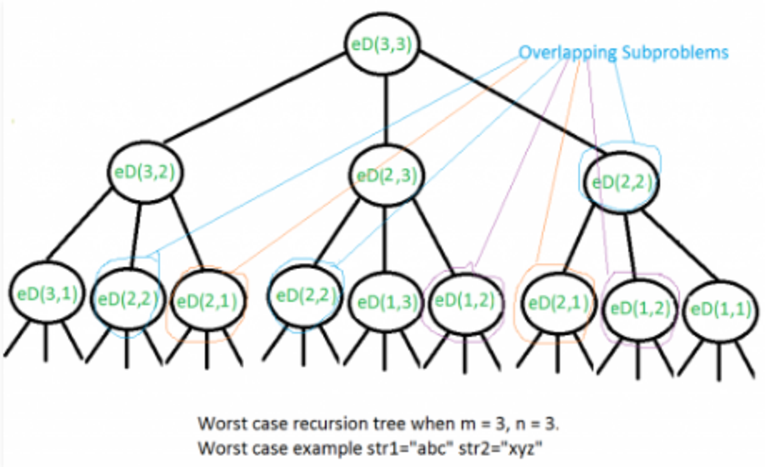
\includegraphics[width=0.7\textwidth]{Images/figGFGDPSet5EditDist}
\label{figGFGDPSet5EditDist}
\end{figure}

We can see that many subproblems are solved again and again, for example
\ctt{eD(2,2)} is called three times. Since same suproblems are called again,
this problem has Overlapping Subprolems property. So Edit Distance problem
has both properties (see this and this) of a dynamic programming problem.
Like other typical Dynamic Programming(DP) problems, recomputations of same
subproblems can be avoided by constructing a temporary array that stores
results of subpriblems.
\begin{lstlisting}[style=raycppnewsnippet]
// A Dynamic Programming based C++ program to find minimum
// number operations to convert str1 to str2
#include<bits/stdc++.h>
using namespace std;
 
// Utility function to find minimum of three numbers
int min(int x, int y, int z)
{
    return min(min(x, y), z);
}

int editDistDP(string str1, string str2, int m, int n)
{
  // Create a table to store results of subproblems
  int dp[m+1][n+1];
 
  // Fill d[][] in bottom up manner
  for (int i=0; i<=m; i++)
  {
    for (int j=0; j<=n; j++)
    {
      // If first string is empty, only option is to
      // isnert all characters of second string
      if (i==0)
          dp[i][j] = j;  // Min. operations = j
 
      // If second string is empty, only option is to
      // remove all characters of second string
      else if (j==0)
          dp[i][j] = i; // Min. operations = i
 
      // If last characters are same, ignore last char
      // and recur for remaining string
      else if (str1[i-1] == str2[j-1])
          dp[i][j] = dp[i-1][j-1];
 
      // If last character are different, consider all
      // possibilities and find minimum
      else
        dp[i][j] = 1 + min(dp[i][j-1],  // Insert
                           dp[i-1][j],  // Remove
                           dp[i-1][j-1]); // Replace
    }
  }
  return dp[m][n];
}
// Driver program
int main()
{
    // your code goes here
    string str1 = "sunday";
    string str2 = "saturday";
 
    cout << editDistDP(str1, str2, str1.length(), str2.length());
 
    return 0;
}
\end{lstlisting}
Output:
\begin{lstlisting}[style=rayio]
3
\end{lstlisting}

\noindent{}\textbf{Time Complexity: O(m x n)}\\
\noindent{}\textbf{Auxiliary Space: O(m x n)}

\textbf{Applications:} There are many practical applications of edit
distance algorithm, refer
Lucene\footnote{\url{http://en.wikipedia.org/wiki/Lucene}} API for sample.
Another example, display all the words in a dictionary that are near
proximity to a given wordincorrectly spelled word.

%%%%%%%%%%%%%%%%%%%%%%%%%%%%%%%%%%%%%%%%%%%%%%%%%%%%%%%%%%%%%%%%%%%%%%%%%%%%
%%%%%%%%%%%%%%%%%%%%%%%%%%%%%%%%%%%%%%%%%%%%%%%%%%%%%%%%%%%%%%%%%%%%%%%%%%%%
%%%%%%%%%%%%%%%%%%%%%%%%%%%%%%%%%%%%%%%%%%%%%%%%%%%%%%%%%%%%%%%%%%%%%%%%%%%%

\section{Dynamic Programming | Set 6 (Min Cost Path)
  \label{secGFGDPSet6MinCostPath}}

\url{http://www.geeksforgeeks.org/dynamic-programming-set-6-min-cost-path/}

\textbf{Difficulty: 2.4}

Given a cost matrix \ctt{cost[][]} and a position $(m, n)$ in
\ctt{cost[][]}, write a function that returns cost of minimum cost path to
reach $(m,n)$ from $(0,0)$. Each cell of the matrix represents a cost to
traverse through that cell. Total cost of a path to reach $(m,n)$ is sum of
all the costs on that path (including both source and destination).
\textbf{You can only traverse \emph{down}, \emph{right} and
  \emph{diagonally} lower cells} from a given cell, i.e., from a given cell
$(i,j)$, cells $(i+1,j)$, $(i,j+1)$ and $(i+1,j+1)$ can be traversed. You
may assume that all costs are positive integers.

For example, in the following figure, what is the minimum cost path to 
$(2,2)$?

\begin{figure}
\centering
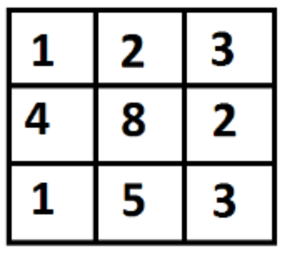
\includegraphics[width=0.2\textwidth]{Images/figGFGDPSet6MinCostPath1}
\label{figGFGDPSet6MinCostPath1}
\end{figure}

The path with minimum cost is highlighted in the following figure. The path
is $(0,0)\to(0,1)\to(1,2)\to(2,2)$. The cost of the path is $8=(1+2+2+3)$.

\begin{figure}
\centering
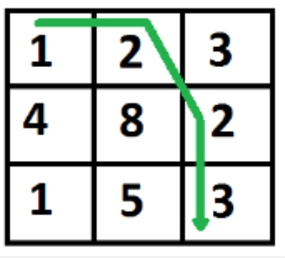
\includegraphics[width=0.2\textwidth]{Images/figGFGDPSet6MinCostPath2}
\label{figGFGDPSet6MinCostPath2}
\end{figure}

\textbf{\rrgreen{Recommended: Please try your approach first, before moving
    on to the solution.}}

\RayNotesBegin

Okay, first we develop the \textbf{optimal substructure}, the
\textbf{states}, and the \textbf{recurrence relation}. How do we go about
this? Remember that we have to try and build the current optimal solution
(in this case to take the min) with a choice of previous optimal solutions.

Say we are at cell $(i,j)$. We could have only reached $(i,j)$ from top
$(i-1,j)$, left $(i,j-1)$ and diagonal $(i-1,j-1)$. \rrhl{These are my three
  actions which I must choose from}. So we have the
recurrence relation:
\begin{equation*}
\text{mC}(i,j)
=\text{c}[i][j]+\min(\text{mC}(i-1,j),\text{mC}(i,j-1),\text{mC}(i-1,j-1))
\end{equation*}
where mC is the minCost function, and c is is the table of costs.
Note that this works because $(i,j)$ depends only on previous solutions.
Otherwise, this problem might get very hard. 

What about base cases and edge cases? The base case (where the recursion
ends) happens at $(i=0,j=0) =\text{c}[0][0]$. For edge cases, we have the
first/top row and the first/left column.
\begin{itemize}%[noitemsep,topsep=0pt]
\item Top row $(i=0,j\neq0)$: cell $(i,j)$ can only be reached from the left
  cell $(i,j-1)$, which gives:
  \begin{equation*}
  \text{mC}(i,j) = \text{c}[i][j]+\text{mC}(i,j-1) \text{ for $i=0,j\neq0$}
  \end{equation*}
\item First column $(i\neq0,j=0)$: cell $(i,j)$ can only be reached from the
  top cell $(i-1,j)$, which gives:
  \begin{equation*}
  \text{mC}(i,j) = \text{c}[i][j]+\text{mC}(i-1,j) \text{ for $i\neq0,j=0$}
  \end{equation*}
\end{itemize}
Now let's code this up. Code found here:\\
\path{src/DynamicProgramming/rrrGFGDPSet6MinCostPath.cpp}
\begin{lstlisting}[style=raycppnewsnippet]
template<typename T>
auto minCost(vector<vector<T>>&cost, size_t m, size_t n)
{
  if(m==0 && n==0)
    return cost[m][n];
  if(m==0 && n != 0)
    return cost[m][n] + minCost(cost,m,n-1);
  if(m!=0 && n==0)
    return cost[m][n] + minCost(cost,m-1,n);

  return cost[m][n] + std::min({minCost(cost,m,n-1),    // left
                                minCost(cost,m-1,n),    // top
                                minCost(cost,m-1,n-1)});// diag
}
\end{lstlisting}
Now for the DP version using bottom up with tabulation
\begin{lstlisting}[style=raycppnewsnippet]
template<typename T>
auto minCostDP(vector<vector<T>>&cost, size_t m, size_t n)
{
  // table of min costs
  // since m and n are used to index the cost table directly, they are one
  // smaller the cost table's sizes. So we +1 when we declare it and give 
  // the size.
  vector<vector<T>> mc(m+1,vector<T>(n+1,T{}));

  using vecsz_t = decltype(cost.size());

  // Take care of base case and edge cases:
  mc[0][0] = cost[0][0];

  // first column
  // Note that we need less than or equal to, since these m and n are used
  // to index the vectors directly. I.e. they range from 0 to cost.size()-1
  for(vecsz_t i = 1; i <= m; ++i)
    mc[i][0] = cost[i][0] + mc[i-1][0];
  
  // first row
  for(vecsz_t j = 1; j <= n; ++j)
    mc[0][j] = cost[0][j] + mc[0][j-1];

  // Now we work in row major order, from first row, then 2nd row, etc...
  for(vecsz_t i = 1; i <= m; ++i)
  {
    for(vecsz_t j = 1; j <= n; ++j)
    {
      mc[i][j] = cost[i][j] + std::min({mc[i-1][j],    // top
                                        mc[i][j-1],    // left
                                        mc[i-1][j-1]});// diag
    }
  }
  // Recall that m and n are not the sizes, we use it to directly index, so 
  // we do not take one off, i.e. not mc[m-1][n-1]
  return mc[m][n];
}
\end{lstlisting}

\RayNotesEnd

\textbf{\rrgreen{Back to geeksforgeeks solution.}}

\rrheader{(1) Optimal Substructure}
The path to reach $(m,n)$ must be through one of the 3 cells: $(m-1,n-1)$ or
$(m-1,n)$ or $(m,n-1)$. So minimum cost to reach $(m,n)$ can be written as
``minimum of the 3 cells plus cost$[m][n]$'':
\begin{equation*}
\text{minCost}(m, n)
=\min(\text{minCost}(m-1,n-1),
      \text{minCost}(m-1, n),
      \text{minCost}(m,n-1))
      +cost[m][n]
\end{equation*}

\rrheader{(2) Overlapping Subproblems}
Following is simple recursive implementation of the MCP (Minimum Cost Path)
problem. The implementation simply follows the recursive structure mentioned
above.
\begin{lstlisting}[style=raycppnewsnippet]
/* A Naive recursive implementation of MCP(Minimum Cost Path) problem */
#include<stdio.h>
#include<limits.h>
#define R 3
#define C 3
 
int min(int x, int y, int z);
 
/* Returns cost of minimum cost path from (0,0) to (m, n) in mat[R][C]*/
int minCost(int cost[R][C], int m, int n)
{
   if (n < 0 || m < 0)
      return INT_MAX;
   else if (m == 0 && n == 0)
      return cost[m][n];
   else
      return cost[m][n] + min( minCost(cost, m-1, n-1),
                               minCost(cost, m-1, n), 
                               minCost(cost, m, n-1) );
}
 
/* A utility function that returns minimum of 3 integers */
int min(int x, int y, int z)
{
   if (x < y)
      return (x < z)? x : z;
   else
      return (y < z)? y : z;
}

/* Driver program to test above functions */
int main()
{
   int cost[R][C] = { {1, 2, 3},
                      {4, 8, 2},
                      {1, 5, 3} };
   printf(" %d ", minCost(cost, 2, 2));
   return 0;
}
\end{lstlisting}
It should be noted that the above function computes the same subproblems
again and again. See the following recursion tree, there are many nodes
which apear more than once. Time complexity of this naive recursive solution
is exponential and it is terribly slow.
\begin{lstlisting}[style=raygeneric]
mC refers to minCost()
                                mC(2, 2)
                      /            |           \
                     /             |            \             
             mC(1, 1)           mC(1, 2)             mC(2, 1)
          /     |     \       /     |     \           /     |     \ 
         /      |      \     /      |      \         /      |       \
   mC(0,0) mC(0,1) mC(1,0) mC(0,1) mC(0,2) mC(1,1) mC(1,0) mC(1,1) mC(2,0) 
\end{lstlisting}
So the MCP problem has both properties (see
\pagecref{secGFGDPSet1OverlapSubprob} and
\pagecref{secGFGDPSet2OptimalSubstruct}) of a dynamic programming problem.
Like other typical Dynamic Programming(DP) problems, recomputations of same
subproblems can be avoided by constructing a temporary array \ctt{tc[][]} in
bottom up manner.
\begin{lstlisting}[style=raycppnewsnippet]
/* Dynamic Programming implementation of MCP problem */
#include<stdio.h>
#include<limits.h>
#define R 3
#define C 3
 
int min(int x, int y, int z);
 
int minCost(int cost[R][C], int m, int n)
{
     int i, j;
 
     // Instead of following line, we can use int tc[m+1][n+1] or 
     // dynamically allocate memoery to save space. The following line is
     // used to keep te program simple and make it working on all compilers.
     int tc[R][C];  
 
     tc[0][0] = cost[0][0];
 
     /* Initialize first column of total cost(tc) array */
     for (i = 1; i <= m; i++)
        tc[i][0] = tc[i-1][0] + cost[i][0];
 
     /* Initialize first row of tc array */
     for (j = 1; j <= n; j++)
        tc[0][j] = tc[0][j-1] + cost[0][j];
 
     /* Construct rest of the tc array */
     for (i = 1; i <= m; i++)
        for (j = 1; j <= n; j++)
            tc[i][j] = min(tc[i-1][j-1], 
                           tc[i-1][j], 
                           tc[i][j-1]) + cost[i][j];
 
     return tc[m][n];
}
/* A utility function that returns minimum of 3 integers */
int min(int x, int y, int z)
{
   if (x < y)
      return (x < z)? x : z;
   else
      return (y < z)? y : z;
}
 
/* Driver program to test above functions */
int main()
{
   int cost[R][C] = { {1, 2, 3},
                      {4, 8, 2},
                      {1, 5, 3} };
   printf(" %d ", minCost(cost, 2, 2));
   return 0;
}
\end{lstlisting}
Output
\begin{lstlisting}[style=rayio]
8
\end{lstlisting}
\rrhl{Time Complexity of the DP implementation is} $\comBigOh{mn}$ which is
much better than Naive Recursive implementation.

Asked in:
Amazon\footnote{\url{https://practice.geeksforgeeks.org/company/Amazon/}}

%%%%%%%%%%%%%%%%%%%%%%%%%%%%%%%%%%%%%%%%%%%%%%%%%%%%%%%%%%%%%%%%%%%%%%%%%%%%
%%%%%%%%%%%%%%%%%%%%%%%%%%%%%%%%%%%%%%%%%%%%%%%%%%%%%%%%%%%%%%%%%%%%%%%%%%%%
%%%%%%%%%%%%%%%%%%%%%%%%%%%%%%%%%%%%%%%%%%%%%%%%%%%%%%%%%%%%%%%%%%%%%%%%%%%%

\section{Dynamic Programming | Set 7 (Coin Change)
  \label{secGFGDPSet7CoinChange}}

\url{http://www.geeksforgeeks.org/dynamic-programming-set-7-coin-change}

\textbf{Difficulty: 3.7}

Given a value $N$, if we want to make change for $N$ cents, and we have
infinite supply of each of $S=\brce*{S_1, S_2,\ldots,S_m}$ valued coins,
\rrhl{how many ways can we make the change?} The order of coins doesn't
matter.

For example, for $N=4$ and $S=\brce*{1,2,3}$, there are four solutions:
$\brce*{1,1,1,1}$, $\brce*{1,1,2}$, $\brce*{2,2}$, $\brce*{1,3}$. So output
should be $4$. For $N=10$ and $S=\brce*{2,5,3,6}$, there are five solutions:
$\brce*{2,2,2,2,2}$, $\brce*{2,2,3,3}$, $\brce*{2,2,6}$, $\brce*{2,3,5}$ and
$\brce*{5,5}$. So the output should be $5$.

\textbf{\rrgreen{Recommended: Please try your approach first, before moving
    on to the solution.}}

\RayNotesBegin

Let's look at the examples again. For $N=4$ and $S=\brce*{1,2,3}$, there are
four solutions. However, if we loop through the coins and try to use them
one by one, we get this:
\begin{lstlisting}[style=raygeneric]
1 + totalcom(n=3):
1 + 3*
1 + 2 + 1*
1 + 1 + 2*
1 + 1 + 1 + 1

2 + totalcom(n=2):
2 + 2
2 + 1 + 1*

3 + totalcom(n=1)
3 + 1*
\end{lstlisting}
So there are seven ways, the ones marked by \ctt{*} are... so this is the
incorrect substructure. Apparently, the optimal substructure comes from
integer
partition\footnote{https://en.wikipedia.org/wiki/Partition\_(number\_theory)}.

I'll just continue with the GFG solution, and also with
\url{http://www.algorithmist.com}.

\RayNotesEnd

From \url{http://www.algorithmist.com/index.php/Coin\_Change}

\rrheader{Coin Change}

\textbf{Coin Change} is the problem of finding the number of ways of making
changes for a particular amount of cents, $n$, using a given set of
denominations $d_{1}\ldots d_{m}$. It is a general case of Integer
Partition, and can be solved with dynamic programming. (The Min-Coin
Change\footnote{http://www.algorithmist.com/index.php/Min-Coin\_Change} is a
common variation of this problem.)

\rrheader{Overview}

The problem is typically asked as: If we want to make change of $N$ cents,
and we have infinite supply of each $S=\brce*{S_1,S_2,\ldots,S_m}$ valued
coins, \rrhl{how many ways can we make the change?} (For simplicity's sake,
the order does not matter.)

It is more precisely defined as:
\begin{quotation}
Given an integer $N$ and a set of integers $S=\brce*{S_1,S_2,\ldots,S_m}$,
how many ways can one express $N$ as a linear combination of
$S=\brce*{S_1,S_2,\ldots,S_m}$ with non-negative coefficients? 
\end{quotation}
Mathematically, how many solutions are there to $N=\sum_{k=1..m}x_kS_k$
where $x_k\geq0, k\in\brce*{1..m}$.  For example, for $N=4,
S=\brce*{1,2,3}$, there are four solutions: $\brce*{1,1,1,1}$,
$\brce*{1,1,2}$, $\brce*{2,2}$, $\brce*{1,3}$.

Other common variations on the problem include decision-based questions,
such as:
\begin{itemize}%[noitemsep,topsep=0pt]
\item Is there a solution for $N=\sum_{k=1..m}x_kS_k$ where $x_k\geq0,
  k\in\brce*{1..m}$ (Is there a solution for integer $N$ and a set of
  integers $S=\brce*{S_1,S_2,\ldots,S_m}$?) \rrgreen{(Solution is to check
    if the number of combination of coins is equal to zero. ezpz.)}
\item Is there a solution for $N =\sum_{k=1..m}x_kS_k$ where
  $x_k\geq0,k\in\brce*{1..m}$, $\sum_{k=1..m}x_k\leq T$ (Is there a solution
  for integer $N$) and a set of integers $S=\brce*{S_1,S_2,\ldots,S_m}$ such
  that $\sum_{k=1..m}x_k\leq T$ - using at most $T$ coins)
\end{itemize}

\rrheader{Recursive Formulation}

\textbf{We are trying to count the number of distinct sets.}

The set f solutions for this problem, $C(N,m)$, cn be partitioned into two
sets:
\begin{itemize}%[noitemsep,topsep=0pt]
\item There are those sets that do not contain any $S_m$ and
\item Those sets that contain at least one $S_m$
\end{itemize}
\begin{enumerate}[label=\textbf{\alph*.}]
\item If a solution does not contain $S_m$, then we can solve the subproblem
  of $N$ with $S=\brce*{S_1,S_2,\ldots,S_{m-1}}$, or the solution of
  $C(N,m-1)$.
\item If a solution does contain $S_m$, then we are using at least one
  $S_m$, thus we are now solving the subproblem of $N-S_m$,
  $S=\brce*{S_1,S_2,\ldots,S_m}$. This is $C(N-S_m, m)$.
\end{enumerate}
\rrblue{(This covers all of the possibilities.)} Thus, we can formulate the
following:
\begin{equation*}
C(N,m) = C(N,m-1)+C(N-S_m,m)
\end{equation*}
with the base cases:
\begin{itemize}%[noitemsep,topsep=0pt]
\item $N=0$ (number of ways to make a sum of 0) implies $C(N,m) = 1$ (one
  solution -- we have no money, exactly one way to solve the problem - by
  choosing no coin change, or, more precisely, to choose coin change of $0$)
\item $N<0$ implies $C(N,m)=0$. (negative sum of money, means we took a
  recursive path which leads to no solution, e.g. if we have $N=5$, and we
  choose to let $S_m=10$ be one of the coins) (no solution -- negative sum
  of money. This can happen along a path ending in $C(N-S_m,m)$.)
\item $N=\geq 1, m\leq 0$, (still money left but no change) implies $C(N,m)
  = 0$. (This can happen along a path ending in $C(N,m-1)$.) 
\end{itemize}

Pseudocode:
\begin{lstlisting}[style=pseudostyle]
int count(int n, int m)
{
  // m < 0 for zero indexed programming languages
  if(n<0 || m<=0)
  {
    return 0;
  }
  // needs be checked after n & m, 
  // as if n = 0 and m < 0 then it would return 1, 
  // which should not be the case.
  if(n==0)
  {
    return 1;
  }
  return count(n,m-1)+count(n-S[m],m)
}
\end{lstlisting}


\rrheader{Dynamic Programming}

Note that the recursion satisfies the weak ordering
\begin{equation*}
R(n,m)<R(x,y)\iff n\leq x,m\leq y, (n,m)\neq (x,y).
\end{equation*}
As a result, this satisfies the optimal-substructure property of dynamic
programming.

The result can be computed in $\comBigOh{nm}$ time - the above pseudocode
can easily be modified to contain memoization. It can be also rewritten as:
\begin{lstlisting}[style=pseudostyle]
func count( n, m )

  for i from 0 to n+1
    for j from 0 to m
      if i equals 0
         table[i, j] = 1          
      else if j equals 0
         if i%S[j] equals 0
               table[i, j] = 1  
         else 
               table[i, j] = 0;
      else if S[j] greater than i
         table[i, j] = table[i, j - 1]
      else 
         table[i, j] = table[i - S[j], j] + table[i, j-1]

  return table[n, m-1]
\end{lstlisting}

\rrsepline{}

\textbf{\rrgreen{Back to geeksforgeeks solution.}}

\rrheader{(1) Optimal Substructure}

To count total number solutions, we can divide all set solutions in two
sets.
\begin{enumerate}[label=\textbf{\arabic*.}]
\item Solutions that do not contain $m$th coin (or $S_m$).
\item Solutions that contain at least one $S_m$.
\end{enumerate}
Let count($S[]$, $m$, $n$) be the function to count the number of solutions,
then it can be written as sum of count($S[]$, $m-1$, $n$) and count($S[]$,
$m$, $n-S_m$).

Therefore, the problem has optimal substructure property as the problem can
be solved using solutions to subproblems.

\rrheader{(2) Overlapping Subproblems}

Following is a simple recursive implementation of the Coin Change problem.
The implementation simply follows the recursive structure mentioned above.
\begin{lstlisting}[style=raycppnewsnippet]
#include<stdio.h>
 
// Returns the count of ways we can sum  S[0...m-1] coins to get sum n
int count( int S[], int m, int n )
{
  // If n is 0 then there is 1 solution (do not include any coin)
  if (n == 0)
    return 1;
   
  // If n is less than 0 then no solution exists
  if (n < 0)
    return 0;
 
  // If there are no coins and n is greater than 0, then no solution exist
  if (m <=0 && n >= 1)
    return 0;
 
  // count is sum of solutions (i) including S[m-1] (ii) excluding S[m-1]
  return count( S, m - 1, n ) + count( S, m, n-S[m-1] );
}
 
// Driver program to test above function
int main()
{
  int i, j;
  int arr[] = {1, 2, 3};
  int m = sizeof(arr)/sizeof(arr[0]);
  printf("%d ", count(arr, m, 4));
  getchar();
  return 0;
}
\end{lstlisting}

\RayNotesBegin

This is my version, found in\\
\path{src/DynamicProgramming/rrrGFGDPSet7CoinChange.cpp}
\begin{lstlisting}[style=raycppnewsnippet]
// Recursively return the count = the number of ways to partition a sum of 
// n using coins in S[0..m-1]. Note that m represents the number of types of
// coins, so the valid inputs are [1..m], but when we index the S array, we
// do S[0..m-1].
int count(vector<int>& S, int m, int n)
{
  // If the sum n is less than 0, then no solution exists.
  if(n<0)
    return 0;

  // If n is greater than 0 and there are no coins left, then there is no
  // solution.
  if(n>=1 && m<=0)
    return 0;

  // If n is 0 then there is 1 solution (do not include any coin)
  if(n==0)
    return 1;
  
  // count is the sum of solution (i) including S[m-1] (ii) excluding S[m-1]
  return count(S,m-1,n) + count(S,m,n-S[m-1]);
}
\end{lstlisting}

\RayNotesEnd

It should be noted that the above function computes the same subproblems
again and again. See the following recursion tree for $S=\brce*{1,2,3}$ and
$n=5$. The function $C(\brce*{1}, 3)$ is called two times. If we draw the
complete tree, then we can see that there are many subproblems being called
more than once. \rrhl{Also note that each path of the recursion tree
  corresponds to one attempt at forming} $\bm{N}$ \rrhl{with the coin types,
  ending with one of the base cases. This will cover all possibilities, even
  those which makes no sense (no solution).}
\begin{lstlisting}[style=raygeneric]
C() --> count()
                              C({1,2,3}, 5)                     
                           /                
                         /                                 
             C({1,2,3}, 2)                 C({1,2}, 5)
            /                             /         
           /                             /           
C({1,2,3}, -1)  C({1,2}, 2)        C({1,2}, 3)    C({1}, 5)
               /                 /                /     
             /                  /                /       
    C({1,2},0)  C({1},2)   C({1,2},1) C({1},3)    C({1}, 4)  C({}, 5)
                   /       /        /         /         
                  /       /        /         /        
                .      .  .     .   .     .   C({1}, 3) C({}, 4)
                                               /  
                                              /      
                                             .      .
\end{lstlisting}
Since same suproblems are called again, this problem has Overlapping
Subprolems property. So the Coin Change problem has both properties (see
\pagecref{secGFGDPSet1OverlapSubprob} and
\pagecref{secGFGDPSet2OptimalSubstruct}) of a dynamic programming problem.
Like other typical Dynamic Programming(DP) problems, recomputations of same
subproblems can be avoided by constructing a temporary array \ctt{table[][]}
in bottom up manner.

\rrheader{Dynamic Programming Solution}

\begin{lstlisting}[style=raycppnewsnippet]
#include<stdio.h>
 
int count( int S[], int m, int n )
{
  int i, j, x, y;
 
  // We need n+1 rows as the table is consturcted in bottom up manner using 
  // the base case 0 value case (n = 0)
  int table[n+1][m];
  
  // Fill the enteries for 0 value case (n = 0)
  for (i=0; i<m; i++)
    table[0][i] = 1;
 
  // Fill rest of the table enteries in bottom up manner  
  for (i = 1; i < n+1; i++)
  {
    for (j = 0; j < m; j++)
    {
      // Count of solutions including S[j]
      x = (i-S[j] >= 0)? table[i - S[j]][j]: 0;
 
      // Count of solutions excluding S[j]
      y = (j >= 1)? table[i][j-1]: 0;
 
      // total count
      table[i][j] = x + y;
    }
  }
  return table[n][m-1];
}

// Driver program to test above function
int main()
{
  int arr[] = {1, 2, 3};
  int m = sizeof(arr)/sizeof(arr[0]);
  int n = 4;
  printf(" %d ", count(arr, m, n));
  return 0;
}
\end{lstlisting}
Output:
\begin{lstlisting}[style=raygeneric]
4
\end{lstlisting}

\RayNotesBegin

This is my version, found in\\
\path{src/DynamicProgramming/rrrGFGDPSet7CoinChange.cpp}
\begin{lstlisting}[style=raycppnewsnippet]
// S is the coin types, n is the sum
int countTabu(vector<int> S, int n)
{
  // number of type of coins. Note that to index the S array, we use
  // j = 0..m-1
  auto m = static_cast<int>(S.size());

  // tab{0..n,0..m-1} of number of ways to partition the sum n. The entry
  // tab(i,j-1) is the number of ways to partition i using j coin types.
  // we need n+1 row as the table is constructed in bottom up manner using
  // the base case 0 (that is, sum n = 0), since we include 0, the indices 
  // actually goes from 0..n, which means the size is n+1.
  vector<vector<int>> tab(n+1,vector<int>(m,0));

  // Recall that the base cases are:
  // n == 0, and we still have coins m>=0, we return 1.
  for(int j = 0; j < m; ++j)
  {
    tab[0][j] = 1;
  }

  // Fill in the rest of the entries in a bottom up manner. Remember the 
  // other two base cases, namely:
  // 1) if sum i < 0, tab is equal to 0
  // 2) if coin types m <= 0, there are no coin types left, so no solution.
  // start i = 1, since the base case i=0 is filled already.
  for(int i = 1; i < n+1; ++i)
  {
    for(int j = 0; j < m; ++j)
    {
      // Count of solutions including S[j]
      int x = 0;
      if(i-S[j]>=0)
        x = tab[i-S[j]][j];
      else
        x=0;

      // Count of solutions excluding S[j]
      int y = 0;
      if(j >= 1)
        y = tab[i][j-1];
      else
        y=0;

      // Total count
      tab[i][j] = x+y;
    }
  }
  return tab[n][m-1];
}
\end{lstlisting}

\RayNotesEnd

\rrhl{Time Complexity:} $\comBigOh{mn}$


\rrhl{NOT DONE RRRTODO}

Following is a simplified version of method 2. \rrhl{The auxiliary space
  required here is} $\comBigOh{n}$ \rrhl{only.}
\begin{lstlisting}[style=raycppnewsnippet]
int count( int S[], int m, int n )
{
  // table[i] will be storing the number of solutions for
  // value i. We need n+1 rows as the table is consturcted
  // in bottom up manner using the base case (n = 0)
  int table[n+1];
 
  // Initialize all table values as 0
  memset(table, 0, sizeof(table));
 
  // Base case (If given value is 0)
  table[0] = 1;
 
  // Pick all coins one by one and update the table[] values
  // after the index greater than or equal to the value of the
  // picked coin
  for(int i=0; i<m; i++)
    for(int j=S[i]; j<=n; j++)
      table[j] += table[j-S[i]];
 
  return table[n];
}
\end{lstlisting}


%%%%%%%%%%%%%%%%%%%%%%%%%%%%%%%%%%%%%%%%%%%%%%%%%%%%%%%%%%%%%%%%%%%%%%%%%%%%
%%%%%%%%%%%%%%%%%%%%%%%%%%%%%%%%%%%%%%%%%%%%%%%%%%%%%%%%%%%%%%%%%%%%%%%%%%%%
%%%%%%%%%%%%%%%%%%%%%%%%%%%%%%%%%%%%%%%%%%%%%%%%%%%%%%%%%%%%%%%%%%%%%%%%%%%%

\section{Find minimum number of coins that make a given value
  \label{secGFGDP}}

\url{http://www.geeksforgeeks.org/find-minimum-number-of-coins-that-make-a-change}

\textbf{Difficulty: 2.5}

\textbf{\rrgreen{Recommended: Please try your approach first, before moving
    on to the solution.}}


\url{http://www.algorithmist.com/index.php/Min-Coin\_Change}

RRRTODO

\RayNotesBegin



\RayNotesEnd

\textbf{\rrgreen{Back to geeksforgeeks solution.}}



%%%%%%%%%%%%%%%%%%%%%%%%%%%%%%%%%%%%%%%%%%%%%%%%%%%%%%%%%%%%%%%%%%%%%%%%%%%%
%%%%%%%%%%%%%%%%%%%%%%%%%%%%%%%%%%%%%%%%%%%%%%%%%%%%%%%%%%%%%%%%%%%%%%%%%%%%
%%%%%%%%%%%%%%%%%%%%%%%%%%%%%%%%%%%%%%%%%%%%%%%%%%%%%%%%%%%%%%%%%%%%%%%%%%%%

\section{Dynamic Programming | Set 8 (Matrix Chain Multiplication)
  \label{secGFGDPSet8MatChainMult}}

\url{http://www.geeksforgeeks.org/dynamic-programming-set-8-matrix-chain-multiplication}

\textbf{Difficulty: 4.2}

Given a sequence of matrices, find the most efficient way to multiply these
matrices together. The problem is not actually to perform the
multiplications, but merely to decide in which order to perform the
multiplications.

We have many options to multiply a chain of matrices because matrix
multiplication is associative. In other words, no matter how we parenthesize
the product, the result will be the same. For example, if we had four
matrices $A$, $B$, $C$, and $D$, we would have:
\begin{equation*}
(ABC)D = (AB)(CD) = A(BCD) = \ldots
\end{equation*}
However, the order in which we parenthesize the product affects the number
of simple arithmetic operations needed to compute the product, or the
efficiency. For example, suppose $A$ is a $10\times30$ matrix, $B$ is a
$30\times5$ matrix, and $C$ is a $5\times60$ matrix. Then,
\begin{align*}
(AB)C&=
(10\times30\times5)+(10\times5\times60)=1500+3000=4500 \text{ operations}\\
A(BC)&=
(30\times5\times60)+(10\times30\times60)=9000+18000=27000 \text{ operations}.
\end{align*}
Clearly the first parenthesization requires less number of operations.

Given an array $p[]$ which represents the chain of matrices such that the
$i$th matrix $A_i$ is of dimension $p[i-1]\times p[i]$. We need to write a
function \ctt{MatrixChainOrder()} that should return the minimum number of
multiplications needed to multiply the chain.

\begin{itemize}[noitemsep,topsep=0pt]
\item Input: $p[]=\brce*{40,20,30,10,30}$
\item Output: $26000$
\item There are $4$ matrices of dimensions $40\times20$, $20\times30$,
  $30\times10$ and $10\times30$.
\item Let the input $4$ matrices be $A$, $B$, $C$ and $D$. The minimum
  number of multiplications are obtained by putting parenthesis in following
  way $(A(BC))D \implies 20*30*10 + 40*20*10 + 40*10*30$
\end{itemize}

\begin{itemize}[noitemsep,topsep=0pt]
\item Input: $p[]=\brce*{10,20,30,40,30}$
\item Output: $30000$
\item There are $4$ matrices of dimensions $10\times20$, $20\times30$,
  $30\times40$ and $40\times30$.
\item Let the input $4$ matrices be $A$, $B$, $C$ and $D$. The minimum
  number of multiplications are obtained by putting parenthesis in following
  way $((AB)C)D \implies 10*20*30 + 10*30*40 + 10*40*30$
\end{itemize}

\begin{itemize}[noitemsep,topsep=0pt]
\item Input: $p[]=\brce*{10,20,30}$
\item Output: $6000$
\item There are only two matrices of dimensions $10x20$ and $20x30$. So
  there is only one way to multiply the matrices, cost of which is
  $10*20*30$.
\end{itemize}

\textbf{\rrgreen{Recommended: Please try your approach first, before moving
    on to the solution.}}

\RayNotesBegin

Let's work with the first example:
\begin{itemize}[noitemsep,topsep=0pt]
\item Input: $p[]=\brce*{40,20,30,10,30}$
\item Output: $26000$
\item There are $4$ matrices of dimensions $40\times20$, $20\times30$,
  $30\times10$ and $10\times30$.
\item Let the input $4$ matrices be $A$, $B$, $C$ and $D$. The minimum
  number of multiplications are obtained by putting parenthesis in following
  way $(A(BC))D \implies 20*30*10 + 40*20*10 + 40*10*30$
\end{itemize}

The matrices are:\\
$A_1 = 40\times20, A_2 = 20\times30, A_3 = 30\times10, A_4 = 10\times30$\\
Thus we have
\begin{lstlisting}[style=raygeneric]
        0  1  2  3  4
p[] = [40,20,30,10,30]
\end{lstlisting}
So what we can do is place a separator which determines the top level
multiplication order, i.e.
\begin{lstlisting}[style=raygeneric]
        0  1  2  3  4
p[] = [40,20|30,10,30] => (A1)*(A2A3A4)

        0  1  2  3  4
p[] = [40,20,30|10,30] => (A1A2)*(A3A4)

        0  1  2  3  4
p[] = [40,20,30,10|30] => (A1A2A3)*(A4)
\end{lstlisting}
And we get the min. number of operations from that. We recursively apply
this algorithm, i.e. to determine the min flops of 
\begin{lstlisting}[style=raygeneric]
        0  1  2  3  4
p[] = [40,20|30,10,30] => (A1)*(A2A3A4)
\end{lstlisting}
We would apply the separation to
\begin{lstlisting}[style=raygeneric]
           1  2  3  4
p[] = [...20,30|10,30] => (A2)*(A3A4)

           1  2  3  4
p[] = [...20,30,10|30] => (A2A3)*(A4)
\end{lstlisting}
And get the min from the above choices. From this, we state the recursive
definition. Notice how in in each level of recursion we have to work with
possibly sub sections of $p[]$, we note this with indices $i$ and $j$.
\begin{align*}
&\text{minFlops}(p[],i = 1,j=n) = \\
&\min_{k=i..j}\left\{p[i-1]*p[k]*p[j] + \text{minFlops}(p[],i,k)+
                        \text{minFlops}(p[],k+1,j)\right\}
\end{align*}
What about the base/edge cases? Well, when there is one matrix, there is no
multiplication, so there are no flops. This happens when $i==j$.
Thus we have:
\begin{lstlisting}[style=pseudostyle,numbers=none]
if(i==j) // no multiplication or 1 matrix
  return 0
\end{lstlisting}

Code found in \path{src/DynamicProgramming/rrrGFGDPSet8MatChainMult.cpp}
\begin{lstlisting}[style=raycppnewsnippet]
//       0, 1, 2, 3, 4
// p = [40,20,30,10,30]
// Start with i=1, j=p.size()-1=4
auto matChainMult(vector<int>& p, int i, int j)->int
{
  // If there is only one matrix, return 0 (no flops)
  if(i==j) return 0;

  int minOps = std::numeric_limits<int>::max();

  // separate between 1 and less than j because the last k will be:
  //       0, 1, 2, 3, 4
  // p = [40,20,30,10,30]
  //                k k+1
  for(int k = i; k < j; ++k)
  {
    int flops = p[i-1]*p[k]*p[j] + matChainMult(p,i,k)
                                 + matChainMult(p,k+1,j);
    if(flops<minOps) minOps = flops;
  }
  return minOps;
}
\end{lstlisting}
Now, how do we do it bottom up? Let's say we store the solution to
subproblems in a table $m[][]$, so that $m[1][4]$ is the solution to
$\text{matChainMult}(p,i=1,j=4)$. From the recursion, we know that this only
depends on problems where $i>1$ and $j<6$. Thus we have
\begin{lstlisting}[style=raygeneric]
j 0|1|2|3|4
i ---------
0| | | | | |
1| |B|B|B|A|
2| | | | |B|
3| | | | |B|
4| | | | |B|
\end{lstlisting}
So \ctt{A} depends on those \ctt{B}s. I'm still not getting anywhere. Let's
look at the base case, and work from that. We know that the base case
happens when $i==j$, i.e. chain multiplication of length $1=j-i+1$ (one
matrix), this yields
\begin{lstlisting}[style=raygeneric]
j 0|1|2|3|4
i ---------
0| | | | | |
1| |0| | | |
2| | |0| | |
3| | | |0| |
4| | | | |0|
\end{lstlisting}
Then we can simply build up from this! Where are the locations of length 2?
I.e. $j-i+1 = 2$, what about $3$?:
\begin{lstlisting}[style=raygeneric]
j 0|1|2|3|4
i ---------
0| | | | | |
1| |1|2|3|4|
2| | |1|2|3|
3| | | |1|2|
4| | | | |1|
\end{lstlisting}
How do we loop through all the $1$s, then $2$s, then $3$s, etc..?
\begin{itemize}%[noitemsep,topsep=0pt]
\item length $l=1$: $i=1$ to $i=4=n-0$, and  $j$ as the
  same.
\item length $l=2$: $i=1$ to $i=3=n-1$, and $j=i+1$.
\item length $l=3$: $i=1$ to $i=n-2$, and $j=$???
\end{itemize}
NO, the above bullet points is a silly way to think about it. If we have
$i$, then we know that $j=i+l-1$, since $l$ is the length, there could only
be one other index $j$ such that $j-i + 1 = l$, we can see this from the
diagonal entries of the middle table:
\begin{lstlisting}[style=raygeneric]
j 0|1|2|3|4
i ---------
0| | | | | |
1| |1|2|3|4|
2| | |1|2|3|
3| | | |1|2|
4| | | | |1|
\end{lstlisting}
Here we have $j-i+1 = l = 0+1 = 1$, since $i==j$. Thus re-arranging this we
have $j=l+i-1$. Now we have to figure out the range of $i$. For each length
$l=1..n$, $i = 1..(n-l+1)$. How did I get $(n-l+1)$? Well, I know that
\begin{align*}
l=1, &i=1..4\\
l=2, &i=1..3\\
l=3, &i=1..2\\
l=4, &i=1..1\\
\end{align*}
So my guess is that we'll have to start at $n=4$ and minus something which 
increases, i.e. $n-l$, however, for the first one, $n-l=4-1=3$, which is one
off from $4$. So I just added $1$ on.

So, to put it all together, we loop from
\begin{lstlisting}[style=pseudostyle,numbers=none]
for(l = 2 .. n-1)
{
  for(i = 2 .. n-l+1)
  {
    j = l+i-1
    m[i,j] = infty
    for(k=i .. j-1)
    {
      q = p[i-1]*p[k]*p[j]+m[i,k]+m[k+1,j]
      if(q<m[i,j])
        m[i,j]=q
    }
  }
}
// This might be a bug, GFG says m[1,n-1]
return m[1,n]
\end{lstlisting}
Actually, GFG is correct relative to their implementation. Because they
initialize $m[n][n]$, where $n=p.size()$. Let's look at the relationship:
\begin{lstlisting}[style=raygeneric]
        0  1  2  3  4
p[] = [40,20,30,10,30] -> A1,A2,A3,A4

j 0|1|2|3|4
i ---------
0| | | | | |
1| |1|2|3|4|
2| | |1|2|3|
3| | | |1|2|
4| | | | |1|
\end{lstlisting}
So we only really need space for $m[4][4]$, however, we make enough space
for $m[5][5]$, to account for the zero-th row and column, which is empty,
however, it's for convenience. Thus, when we want to return the min flops,
for the above example we return $m[1,4]$, which is $m[1,n-1]$. So now I'm
ready to code up the bottom-up version!

Code found in \path{src/DynamicProgramming/rrrGFGDPSet8MatChainMult.cpp}
\begin{lstlisting}[style=raycppnewsnippet]
// Matrix Ai has dimension p[i-1]xp[i] for i=1..n
//
//        0  1  2  3  4
//p[] = [40,20,30,10,30] -> A1,A2,A3,A4
//
//Table m:
//j 0|1|2|3|4
//i ---------
//0| | | | | |
//1| |1|2|3|4|
//2| | |1|2|3|
//3| | | |1|2|
//4| | | | |1|
//
//Table m's entries in the above represent the length, it depicts how the
//below algorithm fills in m, i.e. m[i,j] = i implies that i==j and we're 
//dealing with a matrix mult. of length 1, i.e. one matrix. These are NOT 
//the actual values of m. The actual values of m is the min. flops required
//to perform the mult. of chain length j-i+1.
auto matChainMultDP(vector<int>& p)->int
{
  // length of p, so n-1 is the number of matrices to multiply.
  auto n = static_cast<int>(p.size());

  // Base case: i==j, chain of length 1, so there is no multiplication. We
  // would fill the diagonal entries with 0, but this is already done as 
  // part of the initialization.
  vector<vector<int>>m(n,vector<int>(n,0));

  // Loop from length of 2 to n-1
  for(int l=2; l<n; ++l)
  {
    // Loop down the matrix m.
    for(int i = 1; i < n-l+1; ++i)
    {
      // Calculate the j entries such that j-i+1=l.
      int j = l+i-1;

      // Set number of flops in m to max(), then we can minimize it.
      m[i][j] = std::numeric_limits<int>::max();

      // Loop through all possible splits.
      for(int k=i; k < j; ++k)
      {
        int q = p[i-1]*p[k]*p[j] // Top level mult.
                +m[i][k]         // min flops of left section
                +m[k+1][j];      // min flops of right section

        // Does this give a smaller flop count then a previous split?
        if(q<m[i][j]) m[i][j] = q;
      }
    }
  }

  return m[1][n-1];
}

auto main(int, char* [])->int
{

  vector<int> p{40,20,30,10,30};
  //       0, 1, 2, 3, 4
  // p = [40,20,30,10,30]
  // Start with i=1, j=p.size()-1=4
  cout << matChainMult(p,1,p.size()-1) << '\n';

  cout << matChainMultDP(p)<<'\n';

  return 0;
}
\end{lstlisting}

\RayNotesEnd

\textbf{\rrgreen{Back to geeksforgeeks solution.}}

\rrheader{(1) Optimal Substructure:}

A simple solution is to place parenthesis at all possible places, calculate
the cost for each placement and return the minimum value. In a chain of
matrices of size $n$, we can place the first set of parenthesis in $n-1$
ways.  For example, if the given chain is of $4$ matrices. Let the chain be
$ABCD$, then there are 3 ways to place first set of parenthesis outer side:
$(A)(BCD)$, $(AB)(CD)$ and $(ABC)(D)$. So when we place a set of
parenthesis, we divide the problem into subproblems of smaller size.
Therefore, the problem has optimal substructure property and can be easily
solved using recursion.

Minimum number of multiplication needed to multiply a chain of size $n$ =
Minimum of all $n-1$ placements (these placements create subproblems of
smaller size)

\rrheader{(2) Overlapping Subproblems}

Following is a recursive implementation that simply follows the above
optimal substructure property.
\begin{lstlisting}[style=raycppnewsnippet]
/* A naive recursive implementation that simply
  follows the above optimal substructure property */
#include<stdio.h>
#include<limits.h>
 
// Matrix Ai has dimension p[i-1] x p[i] for i = 1..n
int MatrixChainOrder(int p[], int i, int j)
{
  if(i == j)
    return 0;
  int k; // separator
  int min = INT_MAX;
  int count; // min flops
 
  // place parenthesis at different places between first
  // and last matrix, recursively calculate count of
  // multiplications for each parenthesis placement and
  // return the minimum count
  for (k = i; k <j; k++)
  {
    count = MatrixChainOrder(p, i, k) +
            MatrixChainOrder(p, k+1, j) +
            p[i-1]*p[k]*p[j];
 
    if (count < min)
      min = count;
  }
 
  // Return minimum count
  return min;
}

// Driver program to test above function
int main()
{
  int arr[] = {1, 2, 3, 4, 3};
  int n = sizeof(arr)/sizeof(arr[0]);
 
  printf("Minimum number of multiplications is %d ",
                        MatrixChainOrder(arr, 1, n-1));
 
  getchar();
  return 0;
}
\end{lstlisting}
Time complexity of the above na\"ive recursive approach is exponential. It
should be noted that the above function computes the same subproblems again
and again. See the following recursion tree for a matrix chain of size $4$.
The function \ctt{MatrixChainOrder(p,3,4)} is called two times. We can see
that there are many subproblems being called more than once.

\begin{figure}
\centering
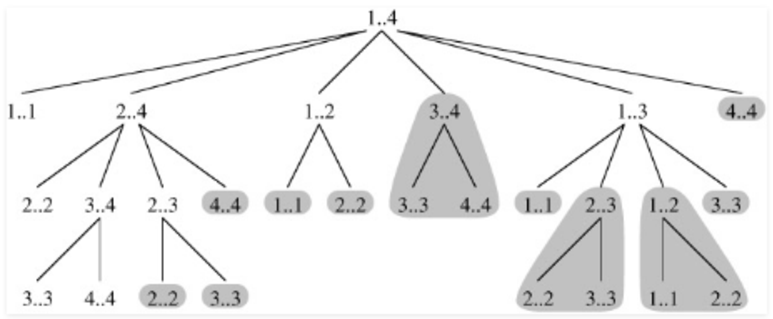
\includegraphics[width=0.7\textwidth]{Images/figGFGDPSet8MatChainMult}
\label{figGFGDPSet8MatChainMult}
\end{figure}

Since same suproblems are called again, this problem has Overlapping
Subprolems property. So Matrix Chain Multiplication problem has both
properties (see \pagecref{secGFGDPSet1OverlapSubprob} and
\pagecref{secGFGDPSet2OptimalSubstruct}) of a dynamic programming problem.
Like other typical Dynamic Programming(DP) problems, recomputations of same
subproblems can be avoided by constructing a temporary array $m[][]$ in
bottom up manner.

\rrheader{Dynamic Programming Solution}

Following is C/C++ implementation for Matrix Chain Multiplication problem
using Dynamic Programming.
\begin{lstlisting}[style=raycppnewsnippet]
// See the Cormen book for details of the following algorithm
#include<stdio.h>
#include<limits.h>
 
// Matrix Ai has dimension p[i-1] x p[i] for i = 1..n
int MatrixChainOrder(int p[], int n)
{
  /* For simplicity of the program, one extra row and one
     extra column are allocated in m[][].  0th row and 0th
     column of m[][] are not used */
  int m[n][n];
 
  int i, j, k, L, q;
 
  /* m[i,j] = Minimum number of scalar multiplications needed
     to compute the matrix A[i]A[i+1]...A[j] = A[i..j] where
     dimension of A[i] is p[i-1] x p[i] */
 
  // cost is zero when multiplying one matrix.
  for (i=1; i<n; i++)
    m[i][i] = 0;
 
  // L is chain length.
  for (L=2; L<n; L++)
  {
    for (i=1; i<n-L+1; i++)
    {
      j = i+L-1;
      m[i][j] = INT_MAX;
      for (k=i; k<=j-1; k++)
      {
        // q = cost/scalar multiplications
        q = m[i][k] + m[k+1][j] + p[i-1]*p[k]*p[j];
        if (q < m[i][j])
          m[i][j] = q;
      }
    }
  }
  return m[1][n-1];
}

int main()
{
    int arr[] = {1, 2, 3, 4};
    int size = sizeof(arr)/sizeof(arr[0]);
 
    printf("Minimum number of multiplications is %d ",
                       MatrixChainOrder(arr, size));
 
    getchar();
    return 0;
}
\end{lstlisting}
Output:
\begin{lstlisting}[style=rayio]
Minimum number of multiplications is 18
\end{lstlisting}
\rrhl{Time Complexity:} $\comBigOh{n^3}$\\
\rrhl{Auxiliary Space:} $\comBigOh{n^2}$

Printing brackets in Matrix Chain Multiplication Problem, see
\pagecref{secGFGDPPrintMatChainMult}.

Please write comments if you find anything incorrect, or you want to share
more information about the topic discussed above.

\subsection{Printing brackets in Matrix Chain Multiplication Problem
  \label{secGFGDPPrintMatChainMult}}

\url{http://www.geeksforgeeks.org/printing-brackets-matrix-chain-multiplication-problem}

\textbf{Difficulty: 4.4}

Given a sequence of matrices, find the most efficient way to multiply these
matrices together. The problem is not actually to perform the
multiplications, but merely to decide in which order to perform the
multiplications.

We have many options to multiply a chain of matrices because matrix
multiplication is associative. In other words, no matter how we parenthesize
the product, the result will be the same. For example, if we had four
matrices A, B, C, and D, we would have:
\begin{lstlisting}[style=raygeneric]
    (ABC)D = (AB)(CD) = A(BCD) = ....
\end{lstlisting}
However, the order in which we parenthesize the product affects the number
of simple arithmetic operations needed to compute the product, or the
efficiency. For example, suppose $A$ is a $10\times30$ matrix, $B$ is a
$30\times5$ matrix, and $C$ is a $5\times60$ matrix. Then,
\begin{equation*}
(AB)C=(10\times30\times5)+(10\times5\times60)=1500+3000=4500
\text{ operations}
\end{equation*}
\begin{equation*}
A(BC)=(30\times5\times60)+(10\times30\times60)=9000+18000=27000 
\text{ operations}.
\end{equation*}
Clearly the first parenthesization requires less number of operations.

Given an array $p[]$ which represents the chain of matrices such that the
$i$th matrix $A_i$ is of dimension $p[i-1]\times p[i]$. We need to write a
function $MatrixChainOrder()$ that should return the minimum number of
multiplications needed to multiply the chain.
\begin{lstlisting}[style=raygeneric]
  Input:  p[] = {40, 20, 30, 10, 30}  
  Output: Optimal parenthesization is  ((A(BC))D)
          Optimal cost of parenthesization is 26000
  There are 4 matrices of dimensions 40x20, 20x30, 30x10 and 10x30.
  Let the input 4 matrices be A, B, C and D.  The minimum number of 
  multiplications are obtained by putting parenthesis in following way
  (A(BC))D --> 20*30*10 + 40*20*10 + 40*10*30

  Input: p[] = {10, 20, 30, 40, 30} 
  Output: Optimal parenthesization is (((AB)C)D)
          Optimal cost of parenthesization is 30000
  There are 4 matrices of dimensions 10x20, 20x30, 30x40 and 40x30. 
  Let the input 4 matrices be A, B, C and D.  The minimum number of 
  multiplications are obtained by putting parenthesis in following way
  ((AB)C)D --> 10*20*30 + 10*30*40 + 10*40*30

  Input: p[] = {10, 20, 30}  
  Output: Optimal parenthesization is (AB)
          Optimal cost of parenthesization is 6000
  There are only two matrices of dimensions 10x20 and 20x30. So there 
  is only one way to multiply the matrices, cost of which is 10*20*30
\end{lstlisting}
This problem is mainly an extension of previous post
\pagecref{secGFGDPSet8MatChainMult}. In the previous post, we have discussed
algorithm for finding optimal cost only. Here we need print parenthssization
also.

\textbf{\rrgreen{Recommended: Please try your approach first, before moving
    on to the solution.}}

\RayNotesBegin

How about, we store the split point in another table, say $brkt[][]$. Let's
play with the example we have been using:
\begin{lstlisting}[style=raygeneric]
        0  1  2  3  4
p[] = [40,20,30,10,30] -> A1,A2,A3,A4

Table m:
j 0|1|2|3|4
i ---------
0| | | | | |
1| |1|2|3|4|
2| | |1|2|3|
3| | | |1|2|
4| | | | |1|

                1  2 3   4
The paren is: ((A1(A2A3))A4)
This means that 
brkt[1,4] = 3
  brkt[1,3] = 1 (left)
    brkt[1,1] = A1 (left)
    brkt[2,3] = 2 (right)
      brkt[2,2] = A2 (left)
      brkt[3,3] = A3 (right)
  brkt[4,4] = A4 right(right)
\end{lstlisting}
This clearly has a recursive structure, and we know that the base case is
when $i==j$, where we just output the matrix name (i.e. $A1$, $A2$, etc...). 
And before each call, we wrap it in brackets.
So the pseudocode would be something like
\begin{lstlisting}[style=pseudostyle,numbers=none]
printParens(brkt[][],i,j)
{
  if(i==j)
  {
    print "Ai"
  }
  else
  {
    print "("
    printParens(brkt,i,brkt[i,j])
    printParens(brkt,brkt[i,j]+1,j)
    print ")"
  }
}
\end{lstlisting}
Now let's code this up!

Code found in \path{src/DynamicProgramming/rrrGFGDPSet8MatChainMult.cpp}
\begin{lstlisting}[style=raycppnewsnippet]
void printParen(vector<vector<int>>&s, int i, int j)
{
  if(i==j)
  {
    cout << "A" << i;
  }
  else
  {
    cout << "(";
    printParen(s,i,s[i][j]);
    printParen(s,s[i][j]+1,j);
    cout << ")";
  }
}

// Matrix Ai has dimension p[i-1]xp[i] for i=1..n
//
//        0  1  2  3  4
//p[] = [40,20,30,10,30] -> A1,A2,A3,A4
//
//Table m:
//j 0|1|2|3|4
//i ---------
//0| | | | | |
//1| |1|2|3|4|
//2| | |1|2|3|
//3| | | |1|2|
//4| | | | |1|
//
//Table m's entries in the above represent the length, it depicts how the
//below algorithm fills in m, i.e. m[i,j] = i implies that i==j and we're 
//dealing with a matrix mult. of length 1, i.e. one matrix. These are NOT 
//the actual values of m. The actual values of m is the min. flops required
//to perform the mult. of chain length j-i+1.
void matChainMultDP(vector<int>& p)
{
  // length of p, so n-1 is the number of matrices to multiply.
  auto n = static_cast<int>(p.size());

  // Base case: i==j, chain of length 1, so there is no multiplication. We
  // would fill the diagonal entries with 0, but this is already done as 
  // part of the initialization.
  vector<vector<int>>m(n,vector<int>(n,0));
  
  // Used to record the split
  vector<vector<int>>s(n,vector<int>(n,0));

  // Loop from length of 2 to n-1
  for(int l=2; l<n; ++l)
  {
    // Loop down the matrix m.
    for(int i = 1; i < n-l+1; ++i)
    {
      // Calculate the j entries such that j-i+1=l.
      int j = l+i-1;

      // Set number of flops in m to max(), then we can minimize it.
      m[i][j] = std::numeric_limits<int>::max();

      // Loop through all possible splits.
      for(int k=i; k < j; ++k)
      {
        int q = p[i-1]*p[k]*p[j] // Top level mult.
                +m[i][k]         // min flops of left section
                +m[k+1][j];      // min flops of right section

        // Does this give a smaller flop count then a previous split?
        if(q<m[i][j])
        {
          m[i][j] = q;
          s[i][j] = k;
        }
      }
    }
  }
  
  cout << "Optimal flops: " << m[1][n-1] << '\n'
       << "With parens: ";
  printParen(s,1,n-1);
  cout << '\n';
}
\end{lstlisting}

\RayNotesEnd

\textbf{\rrgreen{Back to geeksforgeeks solution.}}

The idea is to store optimal break point for every subexpression $(i,j)$ in
a 2D array $bracket[n][n]$. Once we have bracket array us constructed, we
can print parenthesization using below code.
\begin{lstlisting}[style=raycppnewsnippet]
// Prints parenthesization in subexpression (i, j)
printParenthesis(i, j, bracket[n][n], name)
{
  // If only one matrix left in current segment
  if (i == j)
  {
    print name;
    name++;
    return;
  }

  print "(";

  // Recursively put brackets around subexpression
  // from i to bracket[i][j].
  printParenthesis(i, bracket[i][j], bracket, name);

  // Recursively put brackets around subexpression
  // from bracket[i][j] + 1 to j.
  printParenthesis(bracket[i][j]+1, j, bracket, name);

  print ")";
}
\end{lstlisting}

Below is C++ implementation of above steps.
\begin{lstlisting}[style=raycppnewsnippet]
// C++ program to print optimal parenthesization
// in matrix chain multiplication.
#include<bits/stdc++.h>
using namespace std;
 
// Function for printing the optimal
// parenthesization of a matrix chain product
void printParenthesis(int i, int j, int n,
                      int *bracket, char &name)
{
  // If only one matrix left in current segment
  if (i == j)
  {
    cout << name++;
    return;
  }
 
  cout << "(";
 
  // Recursively put brackets around subexpression
  // from i to bracket[i][j].
  // Note that "*((bracket+i*n)+j)" is similar to
  // bracket[i][j]
  printParenthesis(i, *((bracket+i*n)+j), n,
                   bracket, name);
 
  // Recursively put brackets around subexpression
  // from bracket[i][j] + 1 to j.
  printParenthesis(*((bracket+i*n)+j) + 1, j,
                   n, bracket, name);
  cout << ")";
}

// Matrix Ai has dimension p[i-1] x p[i] for i = 1..n
// Please refer below article for details of this
// function
// https://goo.gl/k6EYKj
void matrixChainOrder(int p[], int n)
{
  /* For simplicity of the program, one extra
     row and one extra column are allocated in
      m[][]. 0th row and 0th column of m[][]
      are not used */
  int m[n][n];
 
  // bracket[i][j] stores optimal break point in
  // subexpression from i to j.
  int bracket[n][n];
 
  /* m[i,j] = Minimum number of scalar multiplications
  needed to compute the matrix A[i]A[i+1]...A[j] =
  A[i..j] where dimension of A[i] is p[i-1] x p[i] */
 
  // cost is zero when multiplying one matrix.
  for (int i=1; i<n; i++)
    m[i][i] = 0;
 
  // L is chain length.
  for (int L=2; L<n; L++)
  {
    for (int i=1; i<n-L+1; i++)
    {
      int j = i+L-1;
      m[i][j] = INT_MAX;
      for (int k=i; k<=j-1; k++)
      {
        // q = cost/scalar multiplications
        int q = m[i][k] + m[k+1][j] + p[i-1]*p[k]*p[j];
        if (q < m[i][j])
        {
          m[i][j] = q;
 
          // Each entry bracket[i,j]=k shows
          // where to split the product arr
          // i,i+1....j for the minimum cost.
          bracket[i][j] = k;
        }
      }
    }
  }
  // The first matrix is printed as 'A', next as 'B',
  // and so on
  char name = 'A';
 
  cout << "Optimal Parenthesization is : ";
  printParenthesis(1, n-1, n, (int *)bracket, name);
  cout << "nOptimal Cost is : " << m[1][n-1];
}

// Driver code
int main()
{
  int arr[] = {40, 20, 30, 10, 30};
  int n = sizeof(arr)/sizeof(arr[0]);
  matrixChainOrder(arr, n);
  return 0;
}
\end{lstlisting}

Output:
\begin{lstlisting}[style=rayio]
Optimal Parenthesization: ((A(BC))D)
Minimum Cost of Multiplication: 26000
\end{lstlisting}
\rrhl{Time Complexity:} $O(n^3)$\\
\rrhl{Auxiliary Space:} $O(n^2)$

%%%%%%%%%%%%%%%%%%%%%%%%%%%%%%%%%%%%%%%%%%%%%%%%%%%%%%%%%%%%%%%%%%%%%%%%%%%%
%%%%%%%%%%%%%%%%%%%%%%%%%%%%%%%%%%%%%%%%%%%%%%%%%%%%%%%%%%%%%%%%%%%%%%%%%%%%
%%%%%%%%%%%%%%%%%%%%%%%%%%%%%%%%%%%%%%%%%%%%%%%%%%%%%%%%%%%%%%%%%%%%%%%%%%%%

\section{Dynamic Programming | Set 9 (Binomial Coefficient)
  \label{secGFGDPSet9BinomCoeff}}

\url{http://www.geeksforgeeks.org/dynamic-programming-set-9-binomial-coefficient}

\textbf{Difficulty: 2.5}

Following are common definition of Binomial Coefficients.
\begin{enumerate}[label=\textbf{\arabic*.}]
\item A binomial
  coefficient\footnote{\url{https://en.wikipedia.org/wiki/Binomial\_coefficient}}
  $C(n,k)$ can be defined as the coefficient of $X^k$ in the expansion of
  $(1+X)^n$.
\item A binomial coefficient $C(n,k)$ also gives the number of ways,
  disregarding order, that $k$ objects can be chosen from among $n$ objects;
  more formally, the number of $k$-element subsets (or $k$-combinations
  \rrblue{(order does not matter in $k-$combinations. For a permutation,
    order matters)}) of an $n$-element set.
\end{enumerate}

\rrheader{The Problem}

Write a function that takes two parameters $n$ and $k$ and returns the value
of Binomial Coefficient $C(n,k)$. For example, your function should return
$6$ for $n=4$ and $k=2$, and it should return $10$ for $n=5$ and $k = 2$.

\textbf{\rrgreen{Recommended: Please try your approach first, before moving
    on to the solution.}}

\RayNotesBegin

Err... isn't the binomial coefficient formula:
\begin{equation*}
\binom{n}{k} = \frac{n!}{(n-k)!k!}
\end{equation*}
Let's see, $C(n=5,k=2) = 5!/(3!2!) = 10$

However, if we \emph{had} to use dynamic programming, then we'll need to
come up with a recursive definition which exhibits an optimal substructure
property, and that there are overlapping subproblem.

From the wikipedia article, the recursive formula is
\begin{mdframed}[style=mdfNOTE,
frametitle={Recursive formula from wikipedia}]
\begin{equation*}
\binom{n}{k} = \binom{n-1}{k-1}+\binom{n-1}{k}
\text{ for all integers }n,k:1\leq k \leq n-1,
\end{equation*}
with initial/boundary values
\begin{equation*}
\binom{n}{0} = \binom{n}{n} = 1 \text{ for all integers }n\geq 0.
\end{equation*}
The formula follows from considering the set $\brce*{1,2,\ldots,n}$ and
counting separately
\begin{enumerate}[label=\textbf{\alph*.}]
\item the $k$-element groupings that include a particular set element, say
  ``$i$'', in every group (since ``$i$'' is already chosen to fill one spot
  in every group, we need only choose $k-1$ from the remaining $n-1$) and
\item all the $k$-groupings that don't include ``$i$''; 
\end{enumerate}
this enumerates all the possible $k$-combinations of $n$ elements. It also
follows from tracing the contributions to $X^k$ in $(1+x)^{n-1}(x+x)$. As
there is zero $x^{n+1}$ or $x^{-1}$ in $(1+x)^n$, one might extend the
definition beyond the above boundaries o include $\binom{n}{k}=0$ when
either $k>n$ or $k<0$. This recursive formula then allows the construction
of Pascal's triangle, surrounded by white spaces where the zero, or the
trivial coefficients, would be.
\end{mdframed}

I'm not quite sure that the above means, however the recursive formula can
be seen from Pascal's triangle. However, I get ``It also follows from
tracing the contributions to $X^k$ in $(1+x)^{n-1}(x+x)$.'' Let's look at
Pascal's Triangle:

\begin{tabular}{cccccccccccc}
$n=0$ &&&&&1&&&&    &$(x+y)^0=$&$1$\\
$n=1$ &&&&1&&1&&&   &$(x+y)^1=$&$x+y$\\
$n=2$ &&&1&&2&&1&&  &$(x+y)^2=$&$x^2+2xy+y^2$\\
$n=3$ &&1&&3&&3&&1& &$(x+y)^3=$&$x^3+3x^2y+3xy^2+y^3$\\
$n=4$ &1&&4&&6&&4&&1&$(x+y)^4=$&$x^4+4x^3y+6x^2y^2+4xy^3+y^4$
\end{tabular}

Look how Pascal's Triangle is formed. It's formed by adding the adjacent
digits on the previous row. But we also know that the coefficients of the
binomial are:

\begin{tabular}{cccccccccccc}
$n=0$ &&&&&$\binom{0}{0}$&&&&    &&$1$\\
$n=1$ &&&&$\binom{1}{1}$&&$\binom{1}{0}$&&&   &&$x+y$\\
$n=2$ &&&$\binom{2}{2}$&&$\binom{2}{1}$&&$\binom{2}{0}$&&  &&$x^2+2xy+y^2$\\
$n=3$ &&$\binom{3}{3}$&&$\binom{3}{2}$&&$\binom{3}{1}$&&$\binom{3}{0}$& &&$x^3+3x^2y+3xy^2+y^3$\\
$n=4$
&$\binom{4}{4}$&&$\binom{4}{3}$&&$\binom{4}{2}$&&$\binom{4}{1}$&&$\binom{4}{0}$&&$x^4+4x^3y+6x^2y^2+4xy^3+y^4$
\end{tabular}

As you can see, take $\binom{4}{2}$ for example, the coefficient is clearly
the result of $\binom{3}{2}+\binom{3}{1}$. Of course, you can prove thus by
using the formula $\displaystyle\binom{n}{k} = \frac{n!}{(n-k)!k!}$ and
proving the identity
\begin{equation*}
\binom{n}{k} = \binom{n-1}{k}+\binom{n-1}{k-1}
\end{equation*}

\qasepline{}

Now we can use the recursive definition to do dynamic programming! Given
\begin{equation*}
C(n,k) = C(n-1,k)+C(n-1,k-1)
\end{equation*}
and initial/boundary conditions
\begin{equation*}
C(n,n) = C(n,0) = 1
\end{equation*}
So, let's code his up! Done, code found in:\\
\path{LeetCode/src/DynamicProgramming/rrrGFGDPSet9BinomCoeff.cpp}
\begin{lstlisting}[style=raycppnewsnippet]
unsigned BinomCoeff(unsigned n, unsigned k)
{
  if(k==n || k == 0) return 1;

  if(k>n || k<0) return 0;

  return BinomCoeff(n-1,k)+BinomCoeff(n-1,k-1);
}
void runBinomCoeff(unsigned n, unsigned k)
{
  cout << "C"<<n<<","<<k<<")="<<BinomCoeff(n,k) <<'\n';
}
\end{lstlisting}
Now, how do we do it bottom up? Simples:
\begin{enumerate}[label=\textbf{\arabic*.}]
\item as before, we need a structure to hold the results, let's call this
  $c$. It needs to be 2D because there are two state variables.
\item How do we fill this up? Well, let's do as we did the chain matrix
  mult. We start with a small example and fill in the base case, and see how
  we work up to the final cell.
\end{enumerate}

Let's do $C(n=4,k=3)$. So we have $c=$\\
\begin{tabular}{|c|c|c|c|c|}\hline
\diagbox{$n$}{$k$}&\textbf{0}&\textbf{1}&\textbf{2}&\textbf{3}\\\hline
\textbf{0}&&&&\\\hline 
\textbf{1}&&&&\\\hline
\textbf{2}&&&&\\\hline
\textbf{3}&&&&\\\hline
\textbf{4}&&&&\rrred{4}\\\hline
\end{tabular}\\
where $C(4,3)=4$ (in red) is where we want to get to. First we fill in the
base cases:\\
\begin{tabular}{|c|c|c|c|c|}\hline
\diagbox{$n$}{$k$}&\textbf{0}&\textbf{1}&\textbf{2}&\textbf{3}\\\hline
\textbf{0}&1&&&\\\hline 
\textbf{1}&1&1&&\\\hline
\textbf{2}&1&&1&\\\hline
\textbf{3}&1&&&1\\\hline
\textbf{4}&1&&&\rrred{4}\\\hline
\end{tabular}\\
Now look at the recursion
\begin{equation*}
C(n,k) = \underbrace{C(n-1,k)}_\text{top}+\underbrace{C(n-1,k-1)}_\text{top
left}
\end{equation*}
we know we simply have to loop from $i=2..n$ and $j=1..k-1$. Let's code this
up! Okay, done, this works.
\begin{lstlisting}[style=raycppnewsnippet]
//////////////////////////////////////////////////////////
unsigned BinomCoeffDP(unsigned n, unsigned k)
{
  // Make (n+1)x(k+1) table of 0's
  // we need +1 to account for the zero entry for when we do choose 0 out
  // of n, i.e. C(n,0) = 1.
  auto nrow = n+1;
  auto ncol = k+1;

  vector<vector<unsigned>> dp(nrow,vector<unsigned>(ncol,0));

  // Base case, set C(n,0) = 1, i.e. set the first column to 1's
  for(size_t i = 0; i < nrow; ++i)
  {
    dp[i][0]=1;
  }

  // base case: set C(n,n) to 1, i.e. set the diagonal entries to 1
  for(size_t j = 0; j < ncol; ++j)
  {
    dp[j][j]=1;
  }

  // Calculate binom coeff according to the recursive formula
  // dp[i,j] = dp[i-1,j-1]+dp[i-1,j]
  // See my notes for why I start i = 2 and j=1. It follows from a sketch of
  // dp with the boundary conditions filled only.
  for(size_t i = 2; i <= n; ++i)
  {
    for(size_t j = 1; j <= k; ++j)
    {
      dp[i][j] = dp[i-1][j-1]+dp[i-1][j];
    }
  }

  return dp[n][k];
}
\end{lstlisting}
Code found in:\\
\path{LeetCode/src/DynamicProgramming/rrrGFGDPSet9BinomCoeff.cpp}

\RayNotesEnd

\textbf{\rrgreen{Back to geeksforgeeks solution.}}

\rrheader{(1) Optimal Substructure}

The value of $C(n,k)$ can be recursively calculated using following standard
formula for Binomial Coefficients.
\begin{lstlisting}[style=raygeneric]
C(n, k) = C(n-1, k-1) + C(n-1, k)
C(n, 0) = C(n, n) = 1
\end{lstlisting}
Following is a simple recursive implementation that simply follows the
recursive structure mentioned above.
\begin{lstlisting}[style=raycppnewsnippet]
// A Naive Recursive Implementation
#include<stdio.h>
 
// Returns value of Binomial Coefficient C(n, k)
int binomialCoeff(int n, int k)
{
  // Base Cases
  if (k==0 || k==n)
    return 1;
 
  // Recur
  return  binomialCoeff(n-1, k-1) + binomialCoeff(n-1, k);
}
 
/* Driver program to test above function*/
int main()
{
    int n = 5, k = 2;
    printf("Value of C(%d, %d) is %d ", n, k, binomialCoeff(n, k));
    return 0;
}
\end{lstlisting}

\rrheader{(2) Overlapping Subproblems}

It should be noted that the above function computes the same subproblems
again and again. See the following recursion tree for $n = 5$ and $k = 2$.
The function $C(3,1)$ is called two times. For large values of $n$, there
will be many common subproblems.
\begin{lstlisting}[style=raygeneric]
                             C(5, 2)
                    /                      \
           C(4, 1)                           C(4, 2)
            /   \                          /           \
       C(3, 0)   C(3, 1)             C(3, 1)               C(3, 2)
                /    \               /     \               /     \
         C(2, 0)    C(2, 1)      C(2, 0) C(2, 1)          C(2, 1)  C(2, 2)
                   /        \              /   \            /    \
               C(1, 0)  C(1, 1)      C(1, 0)  C(1, 1)   C(1, 0)  C(1, 1)
\end{lstlisting}
Since same suproblems are called again, this problem has Overlapping
Subproblems property. So the Binomial Coefficient problem has both
properties (see this and this) of a dynamic programming problem. Like other
typical Dynamic Programming(DP) problems, re-computations of same
subproblems can be avoided by constructing a temporary array $C[][]$ in
bottom up manner. Following is Dynamic Programming based implementation.
\begin{lstlisting}[style=raycppnewsnippet]
// A Dynamic Programming based solution that uses table C[][] to
// calculate the Binomial Coefficient
#include<stdio.h>
 
// Prototype of a utility function that returns minimum of two integers
int min(int a, int b);
 
// Returns value of Binomial Coefficient C(n, k)
int binomialCoeff(int n, int k)
{
  int C[n+1][k+1];
  int i, j;
 
  // Caculate value of Binomial Coefficient in bottom up manner
  for (i = 0; i <= n; i++)
  {
    for (j = 0; j <= min(i, k); j++)
    {
      // Base Cases
      if (j == 0 || j == i)
        C[i][j] = 1;
 
      // Calculate value using previosly stored values
      else
        C[i][j] = C[i-1][j-1] + C[i-1][j];
    }
  }
    return C[n][k];
}

// A utility function to return minimum of two integers
int min(int a, int b)
{
  return (a<b)? a: b;
}
 
/* Drier program to test above function*/
int main()
{
  int n = 5, k = 2;
  printf ("Value of C(%d, %d) is %d ", n, k, binomialCoeff(n, k) );
  return 0;
}
\end{lstlisting}
Output:
\begin{lstlisting}[style=rayio]
Value of C[5][2] is 10
\end{lstlisting}

\noindent{}\rrhl{Time Complexity:} $\comBigOh{nk}$\\
\rrhl{Auxiliary Space:} $\comBigOh{nk}$\\

Following is a space optimized version of the above code. The following code
only uses $\comBigOh{k}$. Thanks to AK for suggesting this method.
\begin{lstlisting}[style=raycppnewsnippet]
// C++ program for space optimized Dynamic Programming
// Solution of Binomial Coefficient
#include<bits/stdc++.h>
using namespace std;
 
int binomialCoeff(int n, int k)
{
  int C[k+1];
  memset(C, 0, sizeof(C));

  C[0] = 1;  // nC0 is 1

  for (int i = 1; i <= n; i++)
  {
    // Compute next row of pascal triangle using
    // the previous row
    for (int j = min(i, k); j > 0; j--)
      C[j] = C[j] + C[j-1];
  }
  return C[k];
}
 
/* Driver program to test above function*/
int main()
{
  int n = 5, k = 2;
  printf ("Value of C(%d, %d) is %d ",
          n, k, binomialCoeff(n, k) );
  return 0;
}
\end{lstlisting}
Output:
\begin{lstlisting}[style=rayio]
Value of C[5][2] is 10
Time Complexity: O(n*k)
Auxiliary Space: O(k)
\end{lstlisting}
Explanation:
\begin{lstlisting}[style=raygeneric]
1==========>> n = 0, C(0,0) = 1
1-1========>> n = 1, C(1,0) = 1, C(1,1) = 1
1-2-1======>> n = 2, C(2,0) = 1, C(2,1) = 2, C(2,2) = 1
1-3-3-1====>> n = 3, C(3,0) = 1, C(3,1) = 3, C(3,2) = 3, C(3,3)=1
1-4-6-4-1==>> n = 4, C(4,0) = 1, C(4,1) = 4, C(4,2) = 6, C(4,3)=4, C(4,4)=1
\end{lstlisting}
So here every loop on $i$, builds $i$th row of pascal triangle, using
$(i-1)$th row

At any time, every element of array $C$ will have some value (ZERO or more)
and in next iteration, value for those elements comes from previous
iteration.

In statement,
\begin{lstlisting}[style=raycppnewsnippet]
C[j] = C[j] + C[j-1]
\end{lstlisting}
Right hand side represents the value coming from previous iteration (A row
of Pascal's triangle depends on previous row). Left Hand side represents the
value of current iteration which will be obtained by this statement.
\begin{lstlisting}[style=raygeneric]
Let's say we want to calculate C(4, 3), 
i.e. n=4, k=3:

All elements of array C of size 4 (k+1) are
initialized to ZERO.

i.e. C[0] = C[1] = C[2] = C[3] = C[4] = 0;
Then C[0] is set to 1

For i = 1:
C[1] = C[1] + C[0] = 0 + 1 = 1 ==>> C(1,1) = 1

For i = 2:
C[2] = C[2] + C[1] = 0 + 1 = 1 ==>> C(2,2) = 1
C[1] = C[1] + C[0] = 1 + 1 = 2 ==>> C(2,2) = 2

For i=3:
C[3] = C[3] + C[2] = 0 + 1 = 1 ==>> C(3,3) = 1
C[2] = C[2] + C[1] = 1 + 2 = 3 ==>> C(3,2) = 3
C[1] = C[1] + C[0] = 2 + 1 = 3 ==>> C(3,1) = 3

For i=4:
C[4] = C[4] + C[3] = 0 + 1 = 1 ==>> C(4,4) = 1
C[3] = C[3] + C[2] = 1 + 3 = 4 ==>> C(4,3) = 4
C[2] = C[2] + C[1] = 3 + 3 = 6 ==>> C(4,2) = 6
C[1] = C[1] + C[0] = 3 + 1 = 4 ==>> C(4,1) = 4

C(4,3) = 4 is would be the answer in our example.
\end{lstlisting}
See this for Space and time efficient Binomial Coefficient
\url{http://www.geeksforgeeks.org/space-and-time-efficient-binomial-coefficient/}

RRRTODO

%%%%%%%%%%%%%%%%%%%%%%%%%%%%%%%%%%%%%%%%%%%%%%%%%%%%%%%%%%%%%%%%%%%%%%%%%%%%
%%%%%%%%%%%%%%%%%%%%%%%%%%%%%%%%%%%%%%%%%%%%%%%%%%%%%%%%%%%%%%%%%%%%%%%%%%%%
%%%%%%%%%%%%%%%%%%%%%%%%%%%%%%%%%%%%%%%%%%%%%%%%%%%%%%%%%%%%%%%%%%%%%%%%%%%%

\section{Dynamic Programming | Set 10 (0-1 Knapsack Problem)
  \label{secGFGDPSet10Knapsack01Prob}}

\url{http://www.geeksforgeeks.org/knapsack-problem}

\textbf{Difficulty: 3.3}

Given weights and values of $n$ items, put these items in a knapsack of
capacity $W$ to get the maximum total value in the knapsack. In other words,
given two integer arrays $val[0..n-1]$ and $wt[0..n-1]$ which represent
values and weights associated with $n$ items respectively. Also given an
integer $W$ which represents knapsack capacity, find out the \textbf{maximum
  value} subset of $val[]$ such that \textbf{sum of the weights} of this
subset is smaller than or equal to $W$. You cannot break an item, either
pick the complete item, or don't pick it (0-1 property).

\begin{figure}
\centering
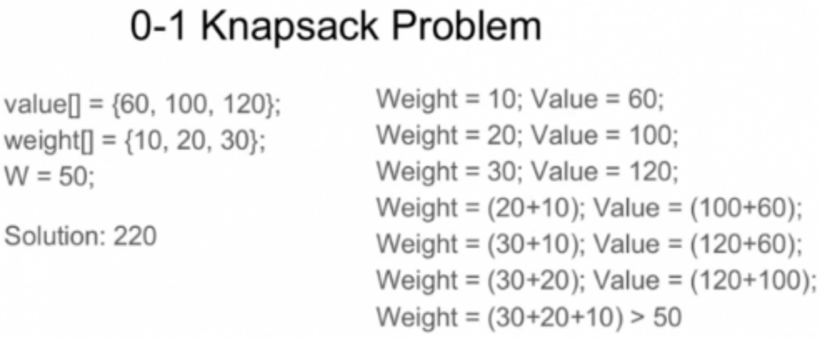
\includegraphics[width=0.7\textwidth]{Images/figGFGDPSet10Knapsack}
\end{figure}

\textbf{\rrgreen{Recommended: Please try your approach first, before moving
    on to the solution.}}

\RayNotesBegin

This is similar to the integer partitioning problem seen in
\pagecref{secGFGDPSet7CoinChange}. In the integer partitioning problem, the
weights and the values have a 1-1 (one to one) mapping. I.e. a value of $5$
has weight $5$. Here, is a more general case where the mapping is defined by
$wt[]$. Thus, we take a similar approach. For each partitioning, we either
use $val[i]$ or we don't. And we must calculate the max weight possible.

Let's start at the right-most val and work backwards, and take a look at
what happens in the two cases:
\begin{lstlisting}[style=raygeneric]
maxWeight(val[],wt[],W,i) = max(maxWeight(val[],wt[],W-wt[i],i  )+val[i]
                                maxWeight(val[],wt[],W,     ,i-1)       )
\end{lstlisting}
If we do use the $val[i]$, then we have the contribution $+val[i]$ to the
knapsack, the resulting subproblem must be of weight $W:=W-wt[i]$. But we're
still using all the values and weights, so $i$ does not change.

If we do not use the weight, in the resulting subproblem, $W$ does not
change, but we reduce the number of weights by 1, hence $i:=i-1$.

This will generate all possible combinations. To see this, consider a small
example: Let $val[]=\brce*{60,100,120}$, $wt[]=\brce*{10,20,30}$ and $W=220$.
Consider what happens if we keep going down the left side of \ctt{max}:
\begin{lstlisting}[style=raygeneric, numbers=left]
       maxWeight(val[],wt[],50,2)
(left) maxWeight(val[],wt[],20,2)+120
(left) maxWeight(val[],wt[],-10,2) END
\end{lstlisting}
This leads to a single val of $120$ with weight $30$ in the bag. But at line
2, instead of going down the left path, if we go down the right path, we
have 
\begin{lstlisting}[style=raygeneric, numbers=left]
       maxWeight(val[],wt[],50,2)
(left) maxWeight(val[],wt[],20,2)+120
(right)maxWeight(val[],wt[],20,1)
(left) maxWeight(val[],wt[],0 ,1)+100
\end{lstlisting}
So we end up with a solution of 220 with $W=0$, this is optimal. What
happens if we keep going to the right?
\begin{lstlisting}[style=raygeneric, numbers=left]
       maxWeight(val[],wt[],50,2)
(right)maxWeight(val[],wt[],50,1)
(right)maxWeight(val[],wt[],50,0)
(right)maxWeight(val[],wt[],50,-1) END
\end{lstlisting}
So we end up with a solution of 0 with $W=50$, this is not a good solution.
However, if in line 3, we take the left path, then we have
\begin{lstlisting}[style=raygeneric, numbers=left]
       maxWeight(val[],wt[],50,2)
(right)maxWeight(val[],wt[],50,1)
(right)maxWeight(val[],wt[],50,0)
(left) maxWeight(val[],wt[],40,0)+60
(left) maxWeight(val[],wt[],30,0)+60
(left) maxWeight(val[],wt[],20,0)+60
(left) maxWeight(val[],wt[],10,0)+60
(left) maxWeight(val[],wt[], 0,0)+60
\end{lstlisting}
So we end up with a solution of 300 with $W=0$, this is even better, and
all we've used are $val=60, wt=10$.

\qasepline{}

The above solution is for when we can pick an item multiple times. If we
cannot pick an item multiple times, then we need a simple modification:
\begin{lstlisting}[style=raygeneric]
maxWeight(val[],wt[],W,i) = max(maxWeight(val[],wt[],W-wt[i],i-1)+val[i]
                                maxWeight(val[],wt[],W,     ,i-1)       )
\end{lstlisting}
On the left path, by adding $i-1$ instead of just $i$, we ensure that once
the item is used, we cannot re-use it. 

Initial and boundary conditions: Since there are two state variables,
logically, there must be four boundary conditions.
\begin{itemize}%[noitemsep,topsep=0pt]
\item If $W=0$, we have no more room, we return $0$ immediately.
\item If $i < 0$, we have no more items, return $0$ immediately.
\item If $W-wt[i]<0$, then we cannot take the weight $wt[i]$ off, we can
  only take the right path (try with a lower weighted item):
\begin{lstlisting}[style=pseudostyle]
if(wt[i]>W)
  return maxWeight(val[],wt[],W,i-1) // go to the right path
\end{lstlisting}
\item Else, we're good to continue taking the max weight:
\begin{lstlisting}[style=pseudostyle]
return max(maxWeight(val[],wt[],W-wt[i],i-1)+val[i],
           maxWeight(val[],wt[],W      ,i-1)        )
\end{lstlisting}
\end{itemize}
Now let's code this up. Aside: I've never known whether I should using a
variable, say $n$, to represent the number of something or whether I could
be using it in terms of an index for a vector. For example:
\begin{lstlisting}[style=raycppnewsnippet]
// i is the number of items, so we need to index with i-1
// i.e. we start counting from 1
void foo(vector<int> v, int i)
{
  vector<int> bar(i);
  auto q = v[i-1];
}
// i is what we use to index a vector, so the caller has to remember to 
// subtract one. I.e. we start counting from 0
void foo(vector<int> v, int i)
{
  vector<int> bar(i+1);
  auto q = v[i];
}
\end{lstlisting}
The former is based 1, the latter is based 0. I'll stick with based 1 for
now since it's more natural. I can hope with fiddling with $-1$ within the
function. In light of this, we have to change our boundary conditions:
\begin{itemize}%[noitemsep,topsep=0pt]
\item If $W=0$, we have no more room, we return $0$ immediately.
\item If $n=0$, we have no more items, return $0$ immediately.
\item If $W-wt[i]<0$, then we cannot take the weight $wt[i]$ ff, we can only
  take the right path (try with a lower weighted item):
\begin{lstlisting}[style=raycppnewsnippet]
if(wt[i]>W)
  return maxWeight(val[],wt[],W,i-1) // go down the right path
\end{lstlisting}
\item Else, we're good to continue taking the max weight:
\begin{lstlisting}[style=raycppnewsnippet]
return max(maxWeight(val[],wt[],W-wt[@Ri-1@],i-1)+val[@Ri-1@],
           maxWeight(val[],wt[],W        ,i-1)          )
\end{lstlisting}
\end{itemize}
Now let's finally code this up. Code found in\\
\path{src/DynamicProgramming/rrrGFGDPSet10Knapsack.cpp}
\begin{lstlisting}[style=raycppnewsnippet]
// Returns the maximum value that can be put in a knapsack of capacity W
template<typename T>
auto knapsack(const vector<T>& val, const vector<T>& wt, 
              const T W, const int n)->T
{
  if(W == 0)
    return 0;
  if(n == 0)
    return 0;

  if(wt[n-1]>W)
    return 0;

  return std::max(knapsack(val,wt,W-wt[n-1],n-1)+val[n-1],
                  knapsack(val,wt,W        ,n-1)          );
}
int main()
{
  {
    vector<int> val{60,100,120};
    vector<int> wt{10,20,30};
    int W = 50;
    int n = val.size();
    cout << knapsack(val,wt,W,n) << '\n';
  }
  return 0;
}
\end{lstlisting}
Now let's do some DP. We know that the state variables are $W$ and $n$, so
let's first define a table to store the results for subproblems:
$dp[W+1][n+1]$,
i.e. this is a $(W+1)\times (n+1)$, where the rows represents all possible
weights (including $0$, hence the $+1$), and the column represents all
possible indices to index the current weight and value. From the recursion:
\begin{lstlisting}[style=raycppnewsnippet]
return max(maxWeight(val[],wt[],@bfW-wt[i-1]@,@bfi-1@)+val[i-1],
           maxWeight(val[],wt[],@bfW@        ,@bfi-1@)          )
\end{lstlisting}
we see that \ctt{dp[i,j]} only depends on the solutions in the top left cell
of $dp$ (due to $(W-wt[i-1],i-1)$) and to the cell on the left (due to
$(W,i-1)$). Thus it's okay to fill $dp$ in row major order from left to
right.

Base cases:\\
\begin{tabular}{|c|c|c|c|c|c|c|}\hline
\diagbox{$W$}{$n$}&\textbf{0}&\textbf{1}&\textbf{2}&\textbf{3}&\textbf{...}&\textbf{n}\\\hline
\textbf{0}&0&0&0&0&0&0\\\hline 
\textbf{1}&0&&&&&\\\hline
\textbf{2}&0&&&&&\\\hline
\textbf{3}&0&&&&&\\\hline
\textbf{4}&0&&&&&\\\hline
\textbf{...}&0&&&&&\\\hline
\textbf{W}&0&&&&&\rrred{ans}\\\hline
\end{tabular}\\
The above table covers the base cases $W=0$ or $n=0$. For the recursive
cases, note that $dp[i,j]$ depends on $dp[i-wt[i],j-1]$ and $dp[i,j-1]$. The
cell $dp[i-wt[i],j-1]$ may not exist if $i-wt[i]<0$, but $dp[i,j-1]$ is
always guaranteed to exist since we only go one to the left, so at most we
hit the base case for $n=0$. Thus, we have to check if $wt[i]>i$ and only
include the solution to the left if so.

Done, code found in \path{src/DynamicProgramming/rrrGFGDPSet10Knapsack.cpp}
\begin{lstlisting}[style=raycppnewsnippet]
template<typename T>
auto knapsackDP(const vector<T>& val, const vector<T>& wt, int W)-> T
{
  using vecsz_t = decltype(val.size());
  // number of items
  auto n = val.size();

  // table for tabulation, +1 for zero entry
  // Note that this also covers the base cases dp[i,j]=0 for i=0 || j=0
  // ALSO NOTE: that when referring to dp, it is "based 1", i.e. if we have 
  // three items,
  // val[]={60, 100, 120}
  // wt[] ={10, 20,  30}
  // Then to refer to the first item, we do val[0], but to refer to the 
  // first item in dp, we do dp[1][1]... hope this makes sense.
  // Also, treat dp as if you were passing state params to a function. So 
  // in the recursive case, it is base 1, so we do it here also.
  // But when referring to the current val, we need to use val[j-1] instead 
  // of just val[j]. Also note that wt is indexed with j, NOT by i which 
  // loops over all weight values.
  vector<vector<T>> dp(W+1,vector<T>(n+1,T{0}));

  for(vecsz_t i = 0; i <= W; ++i)
  {
    for(vecsz_t j = 0; j <= n; ++j)
    {
      if(wt[j-1]>i)
      {
        dp[i][j] = dp[i][j-1];
      }
      else
      {
        dp[i][j] = std::max(dp[i-wt[j-1]][j-1] + val[j-1],
                            dp[i][j-1]);
      }
    }
  }

  return dp[W][n];
}
\end{lstlisting}
I works, let's see the GFG solution.

\RayNotesEnd

\textbf{\rrgreen{Back to geeksforgeeks solution.}}

A simple solution is to consider all subsets of items and calculate the
total weight and value of all subsets. Consider the only subsets whose total
weight is smaller than \rrblue{(or equal to)} $W$. From all such subsets,
pick the maximum value subset.

\rrheader{(1) Optimal Substructure:}

To consider all subsets of items, there can be two cases for every item:
\textbf{(1)} the item is included in the optimal subset, \textbf{(2)} not
included in the optimal set.

Therefore, the maximum value that can be obtained from $n$ items is max of
following two values.
\begin{enumerate}[label=\textbf{\arabic*.}]
\item Maximum value obtained by $n-1$ items and $W$ weight (excluding $n$th
  item).
\item Value of $n$th item plus maximum value obtained by $n-1$ items and $W$
  minus weight of the $n$th item (including $n$th item).
\end{enumerate}

If weight of $n$th item is greater than $W$, then the $n$th item cannot be
included and case 1 is the only possibility.

\rrheader{(2) Overlapping Subproblems}

Following is recursive implementation that simply follows the recursive
structure mentioned above.
\begin{lstlisting}[style=raycppnewsnippet]
/* A Naive recursive implementation of 0-1 Knapsack problem */
#include<stdio.h>
 
// A utility function that returns maximum of two integers
int max(int a, int b) { return (a > b)? a : b; }
 
// Returns the maximum value that can be put in a knapsack of capacity W
int knapSack(int W, int wt[], int val[], int n)
{
  // Base Case
  if (n == 0 || W == 0)
    return 0;
 
  // If weight of the nth item is more than Knapsack capacity W, then
  // this item cannot be included in the optimal solution
  if (wt[n-1] > W)
    return knapSack(W, wt, val, n-1);
 
  // Return the maximum of two cases: 
  // (1) nth item included 
  // (2) not included
  else return max( val[n-1] + knapSack(W-wt[n-1], wt, val, n-1),
                   knapSack(W, wt, val, n-1)
                 );
}
 
// Driver program to test above function
int main()
{
  int val[] = {60, 100, 120};
  int wt[] = {10, 20, 30};
  int  W = 50;
  int n = sizeof(val)/sizeof(val[0]);
  printf("%d", knapSack(W, wt, val, n));
  return 0;
}
\end{lstlisting}
Output:
\begin{lstlisting}[style=rayio]
220
\end{lstlisting}
It should be noted that the above function computes the same subproblems
again and again. See the following recursion tree, $K(1,1)$ is being
evaluated twice. Time complexity of this na\"ive recursive solution is
exponential ($2^n$) \rrblue{(since either an item is included, or it's
  not)}.

In the following recursion tree, $K()$ refers to $knapSack()$.  The two
parameters indicated in the following recursion tree are $n$ and $W$.  The
recursion tree is for following sample inputs.  $wt[] = {1, 1, 1}$, $W = 2$,
$val[] = {10, 20, 30}$
\begin{lstlisting}[style=raygeneric]
                       K(3, 2)         ---------> K(n, W)
                   /            \ 
                 /                \               
            K(2,2)                  K(2,1)
          /       \                  /    \ 
        /           \              /        \
       K(1,2)      K(1,1)        K(1,1)     K(1,0)
       /  \         /   \          /   \
     /      \     /       \      /       \
K(0,2)  K(0,1)  K(0,1)  K(0,0)  K(0,1)   K(0,0)

Recursion tree for Knapsack capacity 2 units and 3 items of 1 unit weight.
\end{lstlisting}
Since suproblems are evaluated again, this problem has Overlapping
Subprolems property. So the 0-1 Knapsack problem has both properties (see
this and this) of a dynamic programming problem. Like other typical Dynamic
Programming(DP) problems, recomputations of same subproblems can be avoided
by constructing a temporary array $K[][]$ in bottom up manner. Following is
Dynamic Programming based implementation.
\begin{lstlisting}[style=raycppnewsnippet]
// A Dynamic Programming based solution for 0-1 Knapsack problem
#include<stdio.h>
 
// A utility function that returns maximum of two integers
int max(int a, int b) { return (a > b)? a : b; }
 
// Returns the maximum value that can be put in a knapsack of capacity W
int knapSack(int W, int wt[], int val[], int n)
{
  int i, w;
  int K[n+1][W+1];
 
  // Build table K[][] in bottom up manner
  for (i = 0; i <= n; i++)
  {
    for (w = 0; w <= W; w++)
    {
      if (i==0 || w==0)
        K[i][w] = 0;
      else if (wt[i-1] <= w)
        K[i][w] = max(val[i-1] + K[i-1][w-wt[i-1]],  K[i-1][w]);
      else
        K[i][w] = K[i-1][w];
    }
  }
 
  return K[n][W];
}
 
int main()
{
  int val[] = {60, 100, 120};
  int wt[] = {10, 20, 30};
  int  W = 50;
  int n = sizeof(val)/sizeof(val[0]);
  printf("%d", knapSack(W, wt, val, n));
  return 0;
}
\end{lstlisting}
Output:
\begin{lstlisting}[style=rayio]
220
\end{lstlisting}
Time Complexity: $\comBigOh{nW}$ where $n$ is the number of items and $W$ is
the capacity of knapsack.

\rrhl{Note that the complexity is always the size of the number of entries
  filled in the table, since we do a constant amount of work per entry of
  the table.}

%01912035626 Angela - health cost?
